\documentclass[11pt]{article}

% Page layout
\usepackage[margin=1in]{geometry}

% Math
\usepackage{amsmath}
\usepackage{amssymb}

% Tables
\usepackage{booktabs}
\usepackage{multirow}
\usepackage{array}

% Graphics and figures
\usepackage{graphicx}
\usepackage{tikz}
\usetikzlibrary{positioning, arrows.meta, calc}

% Colors
\usepackage{xcolor}

% Lists
\usepackage{enumitem}

% Float control
\usepackage{float}

% Code listings
\usepackage{listings}
\lstset{
  basicstyle=\ttfamily\small,
  breaklines=true,
  frame=single,
  columns=fullflexible
}

% Hyperlinks
\usepackage{hyperref}
\hypersetup{
  colorlinks=true,
  linkcolor=blue!60!black,
  citecolor=blue!60!black,
  urlcolor=blue!60!black
}

% Citations
\usepackage{natbib}
\bibliographystyle{plainnat}

% Title
\title{Ploidy: Context-Asymmetric Structured Debate\\for LLM Decision Verification}
\author{heznpc}
\date{}

\begin{document}

\maketitle

% ============================================================
% Abstract
% ============================================================
\begin{abstract}
Single-session LLM usage subjects critical decisions to stochastic prior lock-in: the model's first probabilistic response anchors all subsequent reasoning, and prompt-based mitigations have no statistically significant effect on this bias~\citep{feng2026anchoring}. We present Ploidy, a structured debate protocol between physically separate sessions of the same model with intentionally asymmetric context depths. The framework's primary contributions are conceptual rather than a single headline number: (i)~the distinction between \textbf{Event~A} (context asymmetry---sessions disagree because they have different information) and \textbf{Event~B} (stochastic variance---sessions with identical context disagree due to sampling randomness), which the \emph{ploidy level} (sessions per context depth) controls---confounded at 1n, separable at 2n+; (ii)~the \textbf{Context Asymmetry Spectrum} (Deep~$\to$~Semi-Fresh~$\to$~Fresh) crossed with passive vs.\ active delivery; (iii)~\textbf{context injection mode} (raw, memory, skills, system prompt, CLAUDE.md) as a novel experimental variable for debate efficacy; and (iv)~a \textbf{heterogeneous independence taxonomy} that distinguishes deterministic Fresh (rule-based static analysis) from probabilistic Fresh (zero-context LLM session). Across eight experiments---a six-experiment Phase~1 exploratory study (short- and long-context tasks, ploidy levels 1n--4n, five injection modes, four languages; 1{,}660 valid (task, run, method) triples, primarily on Claude Opus~4.6 with thinner cross-family probes on Sonnet~4.6, Gemini~3.1~Pro, and GPT-5.4) and a pre-registered Phase~2 confirmatory study on nine adversarial tasks (Claude Opus~4.7, Haiku~4.5, Gemini~3.1~Pro) plus a Cross-Challenge ablation---paired Wilcoxon signed-rank tests with Holm--Bonferroni correction support the following observations.

\noindent (1)~The strongest empirical finding is an \emph{inversion} of our initial hypothesis: on the 5 code-review tasks where rule-based static analysis applies, deterministic Tool-Fresh significantly outperforms probabilistic Ploidy (mean $F1 = 0.590$ vs.\ $0.571$, Wilcoxon $p = 0.0098$, $n = 25$ paired comparisons across 5 injection modes $\times$ 5 runs) at one-third the token cost, and Tool-Fresh is stable across all five injection modes ($F1 = 0.559$--$0.617$) while Ploidy varies ($F1 = 0.540$--$0.597$). The source of independence---rule-based vs.\ context-deprived---matters more than its presence.

\noindent (2)~Within the LLM-only baselines that span the same task distribution as Ploidy (no rule-based tools, no domain-mismatch confound), two corrected-significant results hold: Ploidy outperforms Tool+LLM Parallel on recall ($\Delta = +0.414$, $d = 1.13$, $p_\text{corr} < 0.001$, $N = 77$) and F1 ($\Delta = +0.272$, $d = 1.31$, $p_\text{corr} < 0.001$), and Ploidy outperforms unidirectional Cross-Context Review~\citep{song2026ccr} on F1 ($\Delta = +0.054$, $d = 0.53$, $p_\text{corr} = 0.0013$, $N = 95$).

\noindent (3)~Ploidy is statistically \emph{indistinguishable} from Single Session on aggregate recall ($\Delta = -0.001$, $p_\text{corr} = 1.00$, $N = 420$), consistent with the threshold hypothesis that asymmetry helps only when context length crosses an entrenchment regime. On the 3 long-context tasks with anchoring priors, Ploidy shows a directional advantage (4/5 runs, mean $F1 = 0.595$ vs.\ Single $0.565$) but does not reach significance at the per-condition $N$ ($p = 0.44$).

\noindent (4)~Within the long-context per-experiment cells, Ploidy exceeds a Stochastic-N control (matched session count, identical Deep context) by $+0.179$ F1 at 2n on Opus and $+0.192$ F1 at 2n on Codex, suggesting Event~A contributes beyond stochastic sampling. The cross-model sweep further suggests context-asymmetric debate is a high-capability intervention---Ploidy~$>$~Stochastic-N at 4/4 ploidy levels on Opus but reverses on weaker Sonnet, where Fresh sessions appear to inject noise rather than constructive critique. Ploidy~2n is the cost-optimal point on the strongest models at roughly 30\% additional compute over 1n.

\noindent (5)~The remaining open cell---Ploidy~$>$~Single on long-context tasks---is the subject of a pre-registered 4th-sweep replication (\texttt{planning/decisions.md}, 2026-05-21 + 2026-05-27 amendments) whose falsification gates are jointly required on \emph{either} of two co-primary metrics (F1 and recall): $\Delta \bar{M}_{\text{Ploidy}-\text{Single}} \geq 0.030$ where $M \in \{F1, \text{recall}\}$, paired Cohen's $d \geq 0.30$, and Holm--Bonferroni $p_\text{corr} < 0.05$ on $n{=}5 \times 10$ long-context tasks at \texttt{effort=high}, \texttt{injection=raw}, \texttt{lang=en} on Claude Opus 4.7. Two further pre-registered gates harden the run against the known invalidators conceded in \S\ref{sec:limitations}: $\geq 30\%$ of the 10 tasks are drawn from public-record incident post-mortems (\texttt{experiments/src/tasks\_external.py}), and a Cohen's $\kappa \geq 0.40$ secondary-judge agreement gate (\texttt{experiments/src/run\_secondary\_judge.py}) on a 5-task subset re-evaluated by a non-Claude model decides whether the primary judge measurement is trustworthy. A context-length gradient (short $\approx 500$ / medium $\approx 1000$ / long~$=$~full tokens) crosses the 10 base tasks at three lengths to locate the H2 entrenchment threshold (\texttt{tasks\_gradient.py}). Any single gate failing means the data does not support H2 in its current form and the paper is revised accordingly.

\noindent (6)~\textbf{Phase 2 (pre-registered confirmatory).} The Phase~1 nulls above motivated a redesign with explicit bias-vector tasks: nine adversarial tasks across three patterns (authority, ownership, framing). On Opus~4.7, $k{\geq}15$ replications per cell, primary DV = union recall: $H_1$ (ploidy(2n) $>$ single) holds on 9 of 9 tasks, $\Delta = +0.144$, $d = +1.58$, Holm $p_\text{corr} = 0.0059$; $H_4$ (Friedman over 4 methods) holds at $p_\text{corr} = 0.0006$; $H_{10}$ (a heterogeneous-Fresh role-prefix variant) is \emph{strongly rejected} ($\Delta = -0.024$, $d = -1.00$). $H_1$ replicates on Haiku~4.5 ($\Delta = +0.130$, Holm $p_\text{corr} = 0.031$) and directionally on Gemini~3.1~Pro ($n{=}3$ paired, 3/3 positive). An anti-circularity gate (Cohen's $\kappa \geq 0.60$ on a 10\% sub-sample re-judged by gemini-2.5-pro) passes at $\kappa = 0.705$.

\noindent (7)~\textbf{Cross-Challenge ablation.} A pre-registered ablation (\texttt{ploidy\_no\_challenge}: Position $\to$ Convergence, the two cross-challenge calls removed) shows that $\sim89\%$ of the Phase~2 Ploidy lift over Single is delivered by the Position phase alone (NC~$-$~Single $= +0.128$, $d = +1.34$, Wilcoxon $p = 0.0078$); the cross-Challenge phase contributes only $+0.016$ on union recall, indistinguishable from zero ($p = 0.23$). The protocol's named mechanism (Fresh-challenges-Deep / Deep-challenges-Fresh) is therefore null at this DV, and the asymmetric-Position-aggregates-entering-Convergence is where the benefit comes from---a $\sim40\%$ compute reduction is available with negligible recall cost.

\noindent The framework's value lies in defining the experimental design space---context depth, injection mode, independence source, ploidy level---and in producing a pre-registered confirmatory result on a deliberately bias-loaded task pool while honestly reporting the negative ablation finding (cross-Challenge phase null). The intersection of intentional context asymmetry, structured cross-session debate, injection mechanism as experimental variable, ploidy-level stochastic sampling, and heterogeneous independence taxonomy has, to our knowledge, no prior publications as of 2026-05-29.
\end{abstract}

% ============================================================
\section{Introduction}
\label{sec:introduction}
% ============================================================

LLM outputs are stochastic. The same model, given the same prompt, produces different responses across independent sessions. This is well-understood. What is less appreciated is the downstream consequence for single-session workflows:

\begin{enumerate}[label=\arabic*.]
  \item The model's first response is sampled from a probability distribution.
  \item That response enters the context window and becomes the model's own prior.
  \item The model reinforces this prior through consistency-seeking behavior (anchoring bias, sycophancy).
  \item The user sees only one session and treats the output as deterministic.
\end{enumerate}

The result: identical models, identical prompts, identical users---but different project outcomes depending on which stochastic sample landed first. Jacob et al.~\citep{jacob2025chatchamber} term this the ``Chat-Chamber Effect''---the tendency for users to trust and build upon whatever stochastic output a single session produces. This is not addressable by temperature tuning or prompt engineering; empirical evidence shows prompt-based mitigations (chain-of-thought, reflection, ``ignore your prior response'') have no statistically significant effect on anchoring bias~\citep{feng2026anchoring}.

The practical consequence is stark: given the same model and the same prompt, different sessions may produce fundamentally different assessments---agree, disagree, or equivocate---on the same hypothesis. A user confined to a single session is unknowingly subject to a stochastic lottery whose outcome determines not just the quality of individual responses, but whether entire tasks succeed or fail. This extends beyond response quality to task-level outcomes: the same model may complete a task in one session and fail it in another, or require substantially different time to converge, solely due to which stochastic sample anchored the initial response. Two users with identical models and identical problems may experience dramatically different ``model performance'' based solely on which stochastic sample anchored their session.

A natural response is to run multiple sessions and aggregate. But this conflates two independent problems. \textbf{Event~B} (stochastic variance): sessions with identical context disagree because sampling is random---more sessions reduce variance but cannot correct systematic blind spots. \textbf{Event~A} (context-induced bias): a session anchored to accumulated project history has systematic blind spots that no amount of re-sampling from the same context can fix. Running 100 sessions with the same context will converge on the same biased consensus. Only a session with \emph{different} context---one that has never seen the project history---can detect what the context itself has made invisible. This distinction is the core motivation for Ploidy: not more sessions, but sessions with intentionally different information states. The practical importance of this distinction is increasingly recognized: production systems from Anthropic (Agent Teams~\citep{anthropic2026agentteams}), OpenAI (Codex), and Google (Gemini Code Assist) have independently converged on context-isolated multi-agent architectures---but isolate context for parallelism rather than verification, providing no mechanism to control the degree of asymmetry, structure disagreements, or separate Event~A from Event~B (\S\ref{sec:distinction}).

This failure mode is structurally analogous to apoptosis failure in cell biology. The problem is not that the session performs poorly---it is that a session with accumulated errors \emph{does not self-terminate}. It continues generating outputs, the user continues trusting them, and biased conclusions propagate through persistent memory and downstream decisions. A low-performing session that resets is functioning correctly; a high-performing session locked into a biased trajectory is the dangerous case, because its apparent competence masks the accumulated error. Ploidy's Fresh session serves as an external checkpoint---it cannot be anchored to the Deep session's prior outputs, so it detects errors that the Deep session's own context window has rendered invisible.

This pattern has a precise analogue in the history of science. Planck observed that ``a new scientific truth does not triumph by convincing its opponents, but rather because its opponents eventually die, and a new generation grows up that is familiar with it''~\citep{planck1950}. Azoulay et al.~\citep{azoulay2019} provided empirical validation: after the death of eminent scientists, entry by new researchers increases and the field's direction shifts measurably. In both cases, the mechanism is the same---accumulated context (institutional authority, career investment, intellectual commitment) creates systematic blind spots that cannot be corrected from within; only an agent without that context can see what has become invisible. Ploidy operationalizes this principle computationally: the Fresh session is a ``new generation'' that has never been exposed to the Deep session's accumulated priors.

The only computational intervention with empirical support for this problem is physical session separation. Cross-Context Review (CCR)~\citep{song2026ccr}, published concurrently with and independently of this work, demonstrated that a fresh session reviewing an artifact produced by a deep session achieves F1=28.6\% on error detection versus 24.6\% for same-session review ($p=0.008$). CCR validates the core premise that context separation improves review quality. However, CCR is unidirectional---the fresh session reviews but does not debate. Song's follow-up, Dynamic CCR (D-CCR)~\citep{song2026dccr}, tested multi-turn extensions of CCR and found that additional review rounds \emph{degrade} performance: single-pass CCR (F1=0.376) significantly outperformed all multi-turn variants ($p<0.001$), with later rounds introducing false positive pressure and ``Review Target Drift'' where reviewers critique the conversation rather than the artifact. D-CCR's negative result supports our design choice of structured bidirectional debate over iterated unidirectional review---the problem is not insufficient rounds but insufficient \emph{structure} in how disagreements are processed.

Ploidy was developed independently from practical experience with context entrenchment in long-running coding sessions, not derived from CCR or any prior debate framework. Where CCR performs unidirectional review (a fresh session reviews a deep session's artifact), Ploidy uses \textbf{bidirectional structured debate} and introduces the \textbf{Context Asymmetry Spectrum}---a continuum from full context (Deep) through compressed context (Semi-Fresh) to zero context (Fresh). This spectrum recognizes that the optimal information state for a challenger may be neither complete ignorance nor full knowledge, but an intermediate point analogous to the ``experienced outsider'' who brings domain awareness without institutional entrenchment.

\paragraph{Two independent phenomena.} We identify that context asymmetry (Event~A) and stochastic variance (Event~B) are independent events requiring different interventions. A haploid (1n) debate---Deep(1)$\times$Fresh(1)---addresses Event~A but samples only one point from each distribution. Diploid (2n) and higher address both simultaneously: context asymmetry \emph{between} groups, stochastic sampling \emph{within} groups.

\paragraph{Contributions.}
\begin{itemize}[leftmargin=1.5em]
  \item The distinction between Event~A (context asymmetry) and Event~B (stochastic variance) as independently measurable phenomena, controlled by ploidy level (\S\ref{sec:protocol})
  \item A structured debate protocol with typed semantic actions and convergence analysis supporting N-ary sessions (\S\ref{sec:protocol})
  \item Context injection mode (memory, skills, system prompt, raw, CLAUDE.md) as a novel experimental variable for debate efficacy (\S\ref{sec:experiments})
  \item Preliminary evidence suggesting that diploid (2n) may be the cost-optimal ploidy level for recall maximization (\S\ref{sec:experiments})
  \item A pre-registered falsification protocol for the H2 (Context Asymmetry Threshold) replication with effect-size, standardised-effect, significance, external-source, secondary-judge ($\kappa$), and context-length-gradient gates that constrain H2 to a measurable cutoff before any new data is collected (\S\ref{sec:threshold})
  \item An open-source MCP server implementation (\S\ref{sec:implementation})
\end{itemize}

% ============================================================
\section{Background and Related Work}
\label{sec:related}
% ============================================================

\subsection{Context Degradation in Long Sessions}
\label{sec:context-degradation}

LLM performance degrades with context length even when retrieval is perfect---Du et al.~\citep{du2025context} showed 13.9--85\% performance drops that are architectural, not retrieval-related. Chroma Research~\citep{chroma2025contextrot} evaluated 18 frontier models and found effective context capacity is approximately 60--70\% of advertised window size. The ``scaling paradox''~\citep{scaling2026paradox} further shows that larger context compressors produce less faithful reconstructions due to knowledge overwriting. Cheng et al.~\citep{cheng2026contextualdrag} document a complementary failure mode they call \emph{contextual drag}: failed attempts present in the context bias subsequent generations toward structurally similar errors, undermining the assumption that self-improvement pipelines benefit from reflecting on past mistakes. Contextual drag is precisely the failure mode Ploidy's Fresh session is structurally immune to---the Fresh session never sees the Deep session's prior failed attempts, so it cannot inherit their structural error patterns.

\subsection{Multi-Agent Debate}
\label{sec:mad}

Multi-agent debate (MAD) is well-studied but predominantly uses symmetric configurations where all agents share the same context. Recent work has explored multi-LLM context learning for richer discussion dynamics~\citep{m2cl2026}, but the fundamental assumption of shared context remains. Oh et al.~\citep{oh2025dreamad} demonstrated that symmetric debate can amplify bias through ``belief entrenchment.'' Choi et al.~\citep{choi2025debate} proved that debate under symmetric information induces a martingale---it cannot improve expected correctness beyond majority voting. Two recent empirical studies converge on the same conclusion through different methods. Wu et al.~\citep{wu2025reallydebate} ran a controlled study on logical reasoning tasks and found that LLM agents in debate frameworks rarely engage in genuine deliberation beyond ensembling or majority voting. Zhu et al.~\citep{zhu2026demystifying} demystified MAD by isolating its mechanisms and identified two missing ingredients in vanilla MAD that explain why it often underperforms majority vote: \emph{diversity of initial perspectives} and \emph{explicit confidence communication}. Ploidy's context asymmetry is one operationalization of the first ingredient---perspectives diverge structurally from differences in information state rather than from prompt-engineered persona variation. A contemporaneous line of work (SDRL,~\citep{sdrl2026}) addresses the same homogeneous-agent-bias problem through reinforcement learning: a single model is trained on diverse reasoning trajectories derived from multi-agent debate. Ploidy is the inference-time complement---no fine-tuning, and the diversity is sourced from asymmetric context rather than from sampled reasoning paths, which makes the resulting perspectives interpretable as a function of what each session was shown.

ColMAD~\citep{chen2025colmad} reframes debate from competitive zero-sum to collaborative non-zero-sum, where agents critique supportively rather than adversarially, reporting 19\% improvement over competitive MAD. Ploidy shares this collaborative direction through its \texttt{propose\_alternative} and \texttt{synthesize} semantic actions. However, ColMAD and similar collaborative frameworks still operate under symmetric information---all agents share the same context, leaving them vulnerable to collective anchoring. SID~\citep{chen2025sid} drives multi-LLM debate using \emph{self signals} (the model's internal uncertainty estimates) to decide when and how to invoke debate, attempting to lower the cost of debate by selectively triggering it. Ploidy and SID are complementary: SID controls \emph{when} debate fires based on internal signals, Ploidy controls \emph{what asymmetry} the firing debate operates over. Ploidy extends the collaborative paradigm by combining structured semantic actions with intentional context asymmetry.

\subsection{Asymmetric Context as a Mechanism}
\label{sec:asymmetric}

SR-DCR~\citep{srdcr2025} introduced asymmetric context verification debate (ACVD): a context-defending agent debates a context-deprived critic. On GPT-3.5, this achieved 62.7\% accuracy (+3.4pp over naive debate). AceMAD~\citep{liu2026acemad} proved that asymmetric cognitive potential creates submartingale drift toward truth, formally breaking the martingale curse. We note that Ploidy's current single-round design does not satisfy the multi-round conditions required for AceMAD's submartingale proof; whether a multi-round extension would achieve this remains an open question (\S\ref{sec:conclusion}).

AceMAD, concurrent and independent, gives a game-theoretic proof that asymmetric cognitive potential drifts toward truth. Ploidy was developed independently from practical experience with context entrenchment in long-running coding sessions---not from AceMAD's analysis, which we became aware of only at writing time, nor from any game-theoretic motivation. We therefore do not claim that AceMAD grounds Ploidy or that Ploidy validates AceMAD; we report them as independent arrivals at a related insight (that intentional information asymmetry breaks anchoring), one theoretical and one empirical/architectural. Ploidy's distinct contribution is architectural: \emph{what form} of context asymmetry to inject (the Context Asymmetry Spectrum), \emph{how} to deliver it (injection mode), and \emph{how many} sessions separate structural bias from stochastic noise (ploidy level).

\paragraph{Retrieval-side asymmetry analogue.} Courtroom-Style Multi-Agent Debate with Progressive RAG and Role-Switching~\citep{courtroom2026rag} (concurrent, March 2026) attacks the same Echo Chamber problem from the retrieval side: stance-conditioned queries generate distinct evidence pools optimised for supporting and challenging the claim, producing adversarially balanced retrieval. Ploidy and the Courtroom-Style protocol therefore operate on \emph{orthogonal} axes of asymmetry --- Ploidy varies \emph{context depth} between sessions of the same model, the Courtroom protocol varies \emph{retrieved evidence} between roles within a session. Both can compose: a Courtroom-style retrieval policy could feed a Ploidy Deep session while a context-deprived Fresh session reads only the prompt. We leave this composition as future work.

\paragraph{Recently-confirmed prompt-engineering ineffectiveness.} The empirical anchoring-effect study by \citet{anchoring2026synthetic} (arXiv 2505.15392, updated March 2026) confirms that Chain-of-Thought, Reflection, Thoughts-of-Principles, and explicit ``Ignore-Anchor'' instructions \emph{cannot} eliminate LLM anchoring bias --- the bias acts at shallow attention layers that prompt-level interventions do not reach. The same study recommends ``diluting the shallow anchoring influence by providing more balanced contextual signals.'' Ploidy is one operationalisation of that recommendation: the Fresh session is, by construction, a session whose contextual signal is not biased toward the Deep session's accumulated history.

\paragraph{Memory leakage in multi-agent debate.} Multi-Agent Debate with Memory Masking~\citep{mad2026memorymasking} documents that the MAD framework is vulnerable to erroneous memories carried across debate turns and proposes filtering mechanisms. The same failure mode at the \emph{tooling} layer surfaced during the 4th-sweep replication of Ploidy: the underlying Claude Code CLI auto-loads project-memory markdown files into every session, contaminating Fresh seats with fabrication-refusal casebook entries the same model had previously generated. The Memory-Masking work treats this as a within-protocol concern; we treat it as an \emph{infrastructure} concern that pre-experiment review must verify (\S\ref{sec:limitations}, 2026-05-21 incident log).

\subsection{Scaling Agents vs.\ Scaling Diversity}
\label{sec:scaling}

Large-scale agent simulations (e.g., AgentSociety~\citep{pang2025agentsociety} with 10K agents, MiroFish with 700K agents) pursue verification breadth---more agents analyzing the same problem. Boca et al.~\citep{boca2025emergent} showed that even without individual-level bias, LLM populations spontaneously develop collective biases through interaction. Combined with Choi et al.'s martingale result~\citep{choi2025debate}, this suggests that scaling homogeneous agent count does not reliably improve decision quality. Anthropic's own evaluation corroborates: spawning subagents on BrowseComp yielded only +2.8\% over single-agent runs, whereas context management techniques (compaction) produced far larger gains~\citep{anthropic2026harnessing}---improving throughput, not verification depth. Tool augmentation is a third axis: Tool-MAD~\citep{jeong2026toolmad} improves fact verification by giving each debating agent access to diverse retrieval tools and adaptive lookup, but each agent still shares the same anchoring prior because tool retrieval is conditioned on the same context state. Our Tool-Fresh baseline (\S\ref{sec:setup}) implements this design point and is one of the methods Ploidy beats most decisively in the aggregate analysis (\S\ref{sec:aggregate-stats}). Ploidy pursues the orthogonal dimension: verification depth through context diversity.

\subsection{Sycophancy and Persistent Context Bias}
\label{sec:sycophancy}

Jain et al.~\citep{jain2025sycophancy} showed that user memory profiles increase agreement sycophancy by up to 45\% (Gemini~2.5~Pro), with even synthetic contexts causing 15\% uptick. Harshavardhan~\citep{harshavardhan2026sacd} documented self-anchoring calibration drift in multi-turn conversations: Claude Sonnet~4.6 shows significant decreasing confidence under self-anchoring. Laban et al.~\citep{laban2025lost} reported 39\% performance degradation in multi-turn vs.\ single-turn settings, finding that ``when LLMs take a wrong turn, they get lost and do not recover.'' These results motivate Ploidy's Fresh session as a structural reset mechanism.

\subsection{Context Injection as Pseudo-Fine-Tuning}
\label{sec:injection-related}

Context injection and fine-tuning are technically distinct: the former modifies input, the latter modifies weights. Context is ephemeral; fine-tuning is permanent. However, the behavioral boundary is blurring. Persistent context files (CLAUDE.md, memory.md) auto-load every session, functioning as de facto permanent input. In-context learning shifts model behavior to a degree comparable to fine-tuning. RAG pipelines inject external knowledge on every call.

The practical consequence is that developers are \emph{pseudo-fine-tuning} their models through context engineering without recognizing it as such. A memory file that accumulates session observations (``We tried X and it failed'', ``The team decided Y'') causes the model to treat these as internalized knowledge rather than external reference---producing anchoring effects that mimic fine-tuned priors. A skills file with declarative rules (``RULE: always check for X'') is treated as external constraints, producing weaker priors. The \emph{form} of context delivery modulates how strongly the model internalizes it, independently of the information content.

This is why Ploidy treats injection mode as an independent experimental variable: it controls the degree to which context \emph{acts like} fine-tuning. A Fresh session can escape context-induced bias precisely because context is not weight---remove the input and the model reverts. Fine-tuned bias cannot be escaped through session separation.

No prior work treats the delivery mechanism---memory file vs.\ skills file vs.\ system prompt---as an experimental variable for debate outcomes. Vercel~(2026) compared AGENTS.md vs.\ skills for test pass rates; ETH Zurich~(2026) found AGENTS.md files may hinder AI coding agents. Neither connected injection mechanism to anchoring strength or debate efficacy.

\subsection{Model Collapse and Context Contamination}
\label{sec:collapse}

When AI-generated content enters training data, progressive quality degradation occurs---``model collapse''~\citep{shumailov2024collapse}. Ploidy's design of maintaining sessions with different context depths is a within-deployment countermeasure to this homogenization tendency.

\subsection{Positional Bias in Context Delivery}
\label{sec:positional-bias}

LLM attention is non-uniform across the context window. Liu et al.~\citep{liu2023lost} demonstrated a U-shaped performance curve: models attend strongly to information at the beginning and end of the prompt but degrade on middle-positioned content (``Lost in the Middle'' effect). This positional bias is well-established and reflected in official prompt engineering guidelines from both Anthropic and OpenAI.

However, prior multi-agent debate literature has not accounted for how positional bias interacts with debate dynamics. When a compressed summary is injected at the top of a Semi-Fresh prompt (SF-Passive), the model encounters the Deep session's framing \emph{before} the raw artifact---anchoring all subsequent reasoning on that framing. When the same summary is placed at the bottom (SF-Passive-Bottom) or delivered via active retrieval after independent analysis (SF-Active), the positional anchoring is attenuated. Our pilot ablation results are consistent with this mechanism, though confirmation requires larger-scale replication. The contribution is not the discovery of positional bias itself, but the preliminary demonstration that \textbf{context injection architecture may be a moderator variable for multi-agent debate efficacy}---a dimension absent from existing MAD research.

\subsection{Ploidy's Position}
\label{sec:position}

\begin{table}[t]
\centering
\caption{Comparison of Ploidy with prior work along key design dimensions.}
\label{tab:prior-work}
\footnotesize
\setlength{\tabcolsep}{4pt}
\begin{tabular}{@{}p{3.2cm}p{2.4cm}p{3cm}p{2.2cm}p{3cm}@{}}
\toprule
\textbf{Prior Work} & \textbf{Mechanism} & \textbf{Context Depth} & \textbf{Delivery} & \textbf{Direction} \\
\midrule
CCR~\citep{song2026ccr} & Session separation & Binary (Deep/Fresh) & Passive & Unidirectional review \\[3pt]
D-CCR~\citep{song2026dccr} & Multi-turn CCR & Binary (Deep/Fresh) & Passive & Iterated unidirectional (degrades) \\[3pt]
SR-DCR/ACVD~\citep{srdcr2025} & Asymmetric debate & Binary (Defender/Critic) & Passive & Unidirectional + Judge \\[3pt]
AceMAD~\citep{liu2026acemad} & Asymmetric potential & Theoretical & n/a & Multi-round proof \\[3pt]
AgentSociety~\citep{pang2025agentsociety} & Population simulation & Homogeneous & Passive & Observation only \\[3pt]
Agent Teams~\citep{anthropic2026agentteams} & Task division & Independent (same project) & n/a & Coordination (task list) \\[3pt]
\textbf{Ploidy} & \textbf{Structured debate} & \textbf{Spectrum (Deep$\to$Fresh)} & \textbf{Passive + Active} & \textbf{Bidirectional + convergence} \\
\bottomrule
\end{tabular}
\end{table}

\subsection{Distinction from Multi-Agent Task Division}
\label{sec:distinction}

Claude Managed Agents~\citep{anthropic2026managedagents} and similar systems (CrewAI, MetaGPT) implement cooperative division---splitting work across agents for throughput. Adding more agents increases throughput but does not address anchoring bias, because all agents share the same context and thus the same stochastic priors. Under Choi et al.'s martingale result~\citep{choi2025debate}, scaling homogeneous agents is mathematically equivalent to majority voting over identically biased samples.

More recently, production systems have converged on context isolation as a design primitive. Claude Code Agent Teams~\citep{anthropic2026agentteams} gives each teammate an independent context window with coordination through shared task lists and direct messaging. OpenAI Codex runs parallel agents in sandboxed environments. Google Gemini Code Assist supports multi-agent workflows with session separation. Anthropic's desktop redesign~\citep{anthropic2026desktopredesign} further introduces a side-chat mechanism with one-way context flow---the branch reads from the main thread but cannot write back, a pattern structurally analogous to Ploidy's Deep$\to$Fresh information delivery.

This convergence validates the premise that context separation matters for multi-agent quality. However, these systems isolate context \emph{incidentally}---as a side effect of task parallelism---rather than \emph{intentionally} as a mechanism for bias reduction. Agent Teams teammates load the same project context (persistent files, MCP servers, codebase) and coordinate toward task completion, not verification. The isolation is architectural (preventing interference) rather than epistemological (ensuring independent evaluation). No production system provides (1)~controlled variation of context depth across an asymmetry spectrum, (2)~a structured debate protocol with typed semantic actions for processing disagreements, or (3)~causal decomposition of context-induced bias (Event~A) from stochastic variance (Event~B). Ploidy implements the orthogonal strategy: cooperative verification, where the same problem is analyzed from intentionally different information states. The goal is not more output but different perspectives---disagreements are the primary signal, not a failure mode.

\subsection{Commercial Multi-Agent Frameworks (2026-05-29 snapshot)}
\label{sec:industry}

To position Ploidy against the dominant industry framing, we
surveyed the official documentation of six major commercial
multi-agent platforms as of 2026-05-29. Three architectural
patterns emerge:

\textbf{Orchestration / task division.} OpenAI's Agents
SDK~\citep{openai2026agentsdk} provides ``Handoffs'' (explicit
agent-to-agent transfer) and manager-style orchestration over a
sandbox-isolated execution environment; the
sandbox provides filesystem isolation, not
context-asymmetric debate. Microsoft's Agent Framework
v1.0~\citep{microsoft2026agentframework} (updated 2026-04-20)
exposes Agents and graph-based Workflows with type-safe routing,
checkpointing, and human-in-the-loop primitives; the framing is
production engineering---telemetry, state management,
middleware. AWS Bedrock Multi-Agent
Collaboration~\citep{aws2026bedrockmultiagent} (GA 2025, enhanced
2026) implements a hierarchical supervisor-and-collaborators
pattern with task-routing modes. None of these positions
multi-agent as an anti-anchoring mechanism; none decomposes
Event~A from Event~B.

\textbf{Provider interoperability.} Google's Agent-to-Agent
Protocol~\citep{google2025a2a} (announced 2025-04-09, moved to
production at Cloud Next 2026) defines a cross-vendor
communication protocol that 150+ organisations have committed
to. Apple is expected to announce a Siri Extensions
system~\citep{wwdc2026preview} at WWDC 2026 (2026-06-08) that
exposes third-party AI providers (Claude, Gemini, ChatGPT) as
alternative Siri backends. These are interoperability /
distribution patterns; bias-isolation is not a stated goal.

\textbf{Parallel investigation.} Anthropic's Agent
Teams~\citep{anthropic2026agentteams} is the closest commercial
analogue to Ploidy and the one that explicitly acknowledges the
anchoring problem. The official documentation states:
``Sequential investigation suffers from anchoring: once one
theory is explored, subsequent investigation is biased toward
it. With multiple independent investigators actively trying to
disprove each other, the theory that survives is much more
likely to be the actual root cause.'' This is the same
diagnosis Ploidy starts from. But Agent Teams' implementation
keeps the architecture symmetric: each teammate loads the same
project context (CLAUDE.md, MCP servers, skills); the
lead's conversation history does not carry over, but the
\emph{project context}---which is where the anchoring vector
lives---does. There is no structured Position~$\to$~Challenge~$\to$~Convergence
phase machine, no quantitative Event~A / Event~B
decomposition, no Context Asymmetry Spectrum, and no
ablation isolating where the parallel investigation's value
comes from. Ploidy is the natural next step on Anthropic's own
diagnosis: asymmetric context, structured phases, quantified
mechanism (\S\ref{sec:exp7-adversarial}--\S\ref{sec:exp8-ablation}).

\textbf{Summary.} As of 2026-05-29, no commercial multi-agent
framework positions multi-agent as a bias-reduction mechanism
with a quantified decomposition of context-induced from
stochastic variance. Ploidy occupies an empty slot in this
landscape.

% ============================================================
\section{The Ploidy Protocol}
\label{sec:protocol}
% ============================================================

\subsection{The Context Asymmetry Spectrum}
\label{sec:spectrum}

Prior work treats context as binary: full context vs.\ no context. We propose a two-dimensional spectrum defined by \textbf{context depth} and \textbf{context delivery mode}.

\textbf{Context depth} determines how much prior knowledge a session receives:

\begin{figure}[t]
\centering
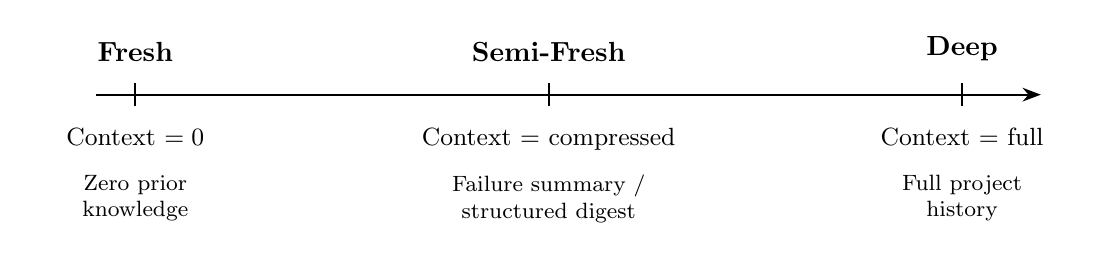
\begin{tikzpicture}[>=Stealth, node distance=0.5cm]
  % Main axis line
  \draw[thick, ->] (0,0) -- (12,0);

  % Tick marks and labels
  \draw[thick] (0.5,-0.15) -- (0.5,0.15);
  \draw[thick] (5.75,-0.15) -- (5.75,0.15);
  \draw[thick] (11,-0.15) -- (11,0.15);

  % Top labels (session names)
  \node[above, font=\bfseries] at (0.5, 0.3) {Fresh};
  \node[above, font=\bfseries] at (5.75, 0.3) {Semi-Fresh};
  \node[above, font=\bfseries] at (11, 0.3) {Deep};

  % Context values
  \node[below, font=\small] at (0.5, -0.3) {Context $= 0$};
  \node[below, font=\small] at (5.75, -0.3) {Context $=$ compressed};
  \node[below, font=\small] at (11, -0.3) {Context $=$ full};

  % Descriptions below
  \node[below, font=\footnotesize, text width=2.5cm, align=center] at (0.5, -0.9) {Zero prior\\knowledge};
  \node[below, font=\footnotesize, text width=3cm, align=center] at (5.75, -0.9) {Failure summary /\\structured digest};
  \node[below, font=\footnotesize, text width=2.5cm, align=center] at (11, -0.9) {Full project\\history};
\end{tikzpicture}
\caption{The Context Depth Spectrum: sessions range from zero prior knowledge (Fresh) through compressed summaries (Semi-Fresh) to full project history (Deep).}
\label{fig:spectrum}
\end{figure}

\begin{itemize}[leftmargin=1.5em]
  \item \textbf{Deep}: Full project context---codebase, decision history, accumulated knowledge. Maximizes domain awareness but risks anchoring bias.
  \item \textbf{Semi-Fresh}: Compressed context---a structured summary of prior attempts, known constraints, or failure modes, without the full narrative that induces entrenchment. Analogous to an experienced outsider or a practitioner restarting a stuck project with lessons learned but freed from sunk-cost attachment.
  \item \textbf{Fresh}: Zero prior context---only the raw artifact under review. Maximizes independence but lacks domain constraints.
\end{itemize}

\textbf{Context delivery mode} determines how context reaches the session, independently of depth:

\begin{itemize}[leftmargin=1.5em]
  \item \textbf{Passive delivery}: Context is embedded directly in the prompt and is always present in the context window. Every response is implicitly influenced by this context, whether or not it is relevant to the specific question being answered. This mirrors the expert whose 20 years of experience unconsciously shapes every judgment.
  \item \textbf{Active delivery}: Context is available through an explicit retrieval mechanism (e.g., a tool call) but is not present in the window until requested. The session must decide when and whether to consult prior knowledge. This mirrors the consultant who researches on demand rather than relying on ingrained assumptions.
\end{itemize}

The same information, delivered passively vs.\ actively, may produce different entrenchment dynamics. This prediction is grounded in established cognitive science findings: the generation effect~\citep{slamecka1978generation} shows that actively produced knowledge is more deeply processed than passively received information, and the testing effect~\citep{roediger2006test} demonstrates that retrieval practice outperforms re-reading for durable learning. Passive delivery maximizes the risk of anchoring bias (the context is always ``priming'' the model), while active delivery introduces a selection step that may reduce entrenchment---the session must formulate a query, which requires some metacognitive awareness of what it does not know. Epley and Gilovich~\citep{epley2006anchoring} showed that anchoring operates through different mechanisms for externally provided vs.\ self-generated anchors, further supporting the prediction that delivery mode matters independently of content.

\begin{figure}[t]
\centering
\caption{The Context Asymmetry Spectrum: a 2D space defined by context depth (rows) and delivery mode (columns), yielding five distinct session configurations.}
\label{fig:2d-matrix}
\vspace{0.5em}
\small
\begin{tabular}{@{} >{\bfseries}l c c c @{}}
\toprule
& \textbf{Passive} & \textbf{Active} & \textbf{None} \\
& \footnotesize(always in window) & \footnotesize(tool/retrieval) & \footnotesize(absent) \\
\midrule
Full
  & Deep & Deep-Active & {\textcolor{gray}{n/a}} \\
  & \footnotesize\textit{(expert intuition)} & \footnotesize\textit{(expert + lookup)} & \\[6pt]
Compressed
  & Semi-Fresh-Passive & Semi-Fresh-Active & {\textcolor{gray}{n/a}} \\
  & \footnotesize\textit{(briefed outsider)} & \footnotesize\textit{(consultant)} & \\[6pt]
None
  & \textcolor{gray}{n/a} & \textcolor{gray}{n/a} & Fresh \\
  & & & \footnotesize\textit{(novice)} \\
\bottomrule
\end{tabular}
\end{figure}

This 2D space yields five distinct session configurations. The current implementation supports Deep (full/passive), Fresh (none), and three Semi-Fresh variants (Passive, Active, Selective) evaluated in \S\ref{sec:exp2}.

\subsection{Architecture}
\label{sec:architecture}

MCP client sessions connect to a single Ploidy server via Streamable HTTP:

\begin{itemize}[leftmargin=1.5em]
  \item \textbf{Deep session}: Full project context (codebase, history, prior decisions)
  \item \textbf{Fresh session}: Only the raw artifact under review (code snippet, architecture question)
  \item \textbf{Semi-Fresh session}: Deep's \textsc{position} output, compressed by a summarization step, as the only context
\end{itemize}

The server maintains debate state in SQLite (WAL mode) and enforces the phase protocol.

\subsection{Ploidy Level}
\label{sec:ploidy-level}

The ploidy level $n$ determines how many sessions are spawned per context depth. At ploidy~1n (haploid), the system runs Deep(1)$\times$Fresh(1)---the minimal asymmetric debate. At ploidy~2n (diploid), it runs Deep(2)$\times$Fresh(2), adding one stochastic backup per depth.

\begin{table}[t]
\centering
\caption{Ploidy levels and their properties.}
\label{tab:ploidy-levels}
\small
\begin{tabular}{@{}llll@{}}
\toprule
\textbf{Ploidy} & \textbf{Sessions} & \textbf{Event A/B} & \textbf{Causal attribution} \\
\midrule
1n (haploid) & Deep$\times$1, Fresh$\times$1 & Confounded & Cannot distinguish \\
2n (diploid) & Deep$\times$2, Fresh$\times$2 & Separable & Within-group $\to$ Event~B \\
3n (triploid) & Deep$\times$3, Fresh$\times$3 & Separable & Majority voting within groups \\
4n+ & Deep$\times$N, Fresh$\times$N & Separable & Statistical significance \\
\bottomrule
\end{tabular}
\end{table}

At 1n, the system cannot distinguish whether a disagreement between Deep and Fresh is caused by context asymmetry (Event~A) or stochastic variance (Event~B). At 2n+, within-group disagreement isolates Event~B (both Deep sessions had identical context, so any disagreement is stochastic), while between-group disagreement isolates Event~A. The ploidy level trades compute cost for causal interpretability.

\subsection{Context Injection Modes}
\label{sec:injection-modes}

The same context information can be delivered to the Deep session in different formats, each creating different anchoring dynamics:

\begin{table}[t]
\centering
\caption{Context injection modes.}
\label{tab:injection-modes}
\small
\begin{tabular}{@{}lp{8cm}@{}}
\toprule
\textbf{Mode} & \textbf{Description} \\
\midrule
\texttt{raw} & Plain text in user prompt (baseline) \\
\texttt{memory} & Accumulated observations as numbered items (CLAUDE.md style) \\
\texttt{skills} & Declarative rules and constraints (skills.md style) \\
\texttt{system\_prompt} & Context via system-level instruction \\
\texttt{claude\_md} & XML-tagged project instructions \\
\bottomrule
\end{tabular}
\end{table}

The hypothesis is that narrative context (memory) creates stronger anchoring priors than declarative context (skills), because the model treats ``learned observations'' as internalized beliefs rather than external constraints.

\subsection{Debate Phases}
\label{sec:phases}

\begin{enumerate}[label=\arabic*., leftmargin=1.5em]
  \item \textbf{Position}: All sessions independently analyze the artifact. Each produces a list of findings with confidence levels.
  \item \textbf{Challenge}: Each session reviews the others' positions. For each finding, the reviewer responds with a typed semantic action:
  \begin{itemize}[leftmargin=1em]
    \item \texttt{agree}---finding is valid
    \item \texttt{challenge}---finding is wrong or misleading, with explanation
    \item \texttt{propose\_alternative}---finding is partially right, here's a different framing
    \item \texttt{synthesize}---combining both perspectives into a stronger finding
  \end{itemize}
  \item \textbf{Convergence}: The protocol analyzes the debate transcript and classifies outcomes:
  \begin{itemize}[leftmargin=1em]
    \item \textbf{Agreements}: findings confirmed by multiple sessions
    \item \textbf{Productive disagreements}: findings where challenge/synthesis produced new insight
    \item \textbf{Irreducible disagreements}: genuine differences that could not be resolved
    \item \textbf{Confidence score}: proportion of agreed findings
  \end{itemize}
\end{enumerate}

\subsection{Design Principles}
\label{sec:principles}

\begin{itemize}[leftmargin=1.5em]
  \item \textbf{No shared memory}: Fresh/Semi-Fresh sessions never see Deep's raw analysis outside the debate protocol.
  \item \textbf{Typed actions over free-form}: Semantic actions make the debate transcript machine-interpretable.
  \item \textbf{Disagreement as signal}: Irreducible disagreements are informative, not failures---they mark where context mattered.
\end{itemize}

% ============================================================
\section{Implementation}
\label{sec:implementation}
% ============================================================

Ploidy is implemented as a Python MCP server (FastMCP, asyncio, aiosqlite) exposing 11 tools over Streamable HTTP on port 8765. The server manages debate lifecycle, enforces phase transitions via a finite state machine (\textsc{independent} $\to$ \textsc{position} $\to$ \textsc{challenge} $\to$ \textsc{convergence} $\to$ \textsc{complete}), and persists all state in SQLite with WAL mode and foreign key cascades for crash recovery. Per-debate asyncio locks guard concurrent phase transitions; API calls retry with exponential backoff on transient failures.

\paragraph{v0.3 enhancements.} Building on v0.2 (Semi-Fresh sessions, API fallback, LLM convergence, dashboard), v0.3 adds:
\begin{itemize}[leftmargin=1.5em]
  \item \textbf{Cross-model validation}: Experiment runner supporting 4 backends (Anthropic, OpenAI, Ollama/Codex, Gemini) with Stochastic-N baselines for Event~A/B isolation (\S\ref{sec:cross-model}).
  \item \textbf{Human-in-the-loop} (\texttt{debate\_review}): The \texttt{debate\_auto} tool now accepts a \texttt{pause\_at} parameter (``challenge'' or ``convergence'') that pauses the automated debate for human review. The reviewer can approve, override (replacing auto-generated content), or reject the debate via the new \texttt{debate\_review} tool---closing the gap between fully-automated and fully-manual workflows.
  \item \textbf{Effort level}: Configurable reasoning depth parameter that controls how much computation the model applies per response---an experimental variable that may interact with context asymmetry (\S\ref{sec:effort}).
  \item \textbf{Sweep infrastructure}: Ploidy-level (1n--4n), effort (low/high/max), injection mode (raw/memory/skills/system\_prompt/claude\_md), and language (en/ko/ja/zh) sweeps with 25 extended tasks.
\end{itemize}

We note that the experiments in \S\ref{sec:experiments} use the \texttt{claude --print} CLI to simulate the protocol rather than the MCP server directly, as this provides cleaner session isolation for controlled comparison. Each CLI invocation creates a guaranteed-fresh session with no shared state. The MCP server is designed for production use where two human-operated terminals connect to the same server instance.

\paragraph{Service vs research surfaces.} The 11-tool phase-state surface described above is the \emph{research protocol}: it exposes every phase transition so experiment runners can exercise context asymmetry under tight control. For service usage we additionally ship a single \texttt{debate(prompt, mode=...)} tool (see \texttt{src/ploidy/server.py}) that collapses the state machine into one call, and a companion \texttt{/ploidy} Claude Code slash command (\texttt{.claude/commands/ploidy.md}) that automates the deep vs fresh sub-agent orchestration. The legacy 11-tool surface remains canonical for the experiments reported here.

\paragraph{Reproducibility.} The numbers reported in \S\ref{sec:experiments} were produced by \texttt{experiments/src/run\_experiment.py}, which uses the \texttt{claude --print} CLI and its own inline prompts; it does not depend on the MCP service code path. To reproduce exactly, check out the \texttt{v0.3.3-paper} git tag. Subsequent service-layer commits (v0.4+) introduced caching-oriented prompt rewrites in \texttt{src/ploidy/api\_client.py} that do not touch the experimental pipeline but would affect anyone comparing service-mode outputs to the paper's numbers.

\paragraph{Raw artefact availability.} The per-(task, method, run) result JSONs underlying the 1\,660-entry aggregate analysis are stored under \texttt{experiments/results/}, which is gitignored locally because the directory is large and regenerable from the runner. A \emph{manifest} of those runs — one summary record per Claude Code session that produced the outputs — is committed to the repository at \texttt{experiments/data/processed/claude\_sessions/INDEX.json} (machine-readable) and \texttt{INDEX.md} (human-readable). For the 4th-sweep replication that resolves the remaining open cell (\S\ref{sec:threshold}), the raw \texttt{results/} tree will be bundled into the Zenodo deposit alongside the \texttt{v0.3.4-paper} tag so reviewers can verify the pipeline end-to-end without re-running the model calls.

Full source: \url{https://github.com/heznpc/ploidy-research}

% ============================================================
\section{Experiments}
\label{sec:experiments}
% ============================================================

\paragraph{Evidence level.} The following results are from pilot experiments designed to validate the protocol's feasibility and identify promising directions. Sample sizes are insufficient for statistical inference: most experiments use single runs across 3--10 tasks, and observed effect sizes are smaller than within-method stochastic variance. We present these observations to motivate the research direction and invite replication with larger samples. No claim in this section should be read as a statistically validated finding.

This section reports preliminary pilot results. All findings should be interpreted as observations from a small-scale pilot study, not as statistically validated conclusions. We report both null and positive observations to bound where context asymmetry applies.

\subsection{Setup}
\label{sec:setup}

We evaluate on 10 tasks across two context regimes:
\begin{itemize}[leftmargin=1.5em]
  \item \textbf{Experiment~1} (short context, $\sim$50 tokens): 5 code review tasks with injected bugs + 2 architecture decision tasks. Each has 3--5 ground-truth issues.
  \item \textbf{Experiment~2} (long context, 2,000--5,000 tokens): 3 architecture decision tasks with project histories containing anchoring-inducing biases. Each has 5--6 ground-truth issues.
\end{itemize}

\paragraph{Model transition mid-program.} Experiments~1 through~3 (the original sweeps that produced 1{,}601 of the 1{,}660 aggregate entries, dated 2026-03-18 through 2026-04-17) ran on \textbf{Claude Opus 4.6}. From 2026-04-23 onward (the long-context $n{=}5$ replication and the 4th-sweep replication described in \S\ref{sec:threshold}) we transitioned to \textbf{Claude Opus 4.7} with the expanded 1M-token context window. The 59 entries in the aggregate analysis from 2026-04-23 forward are therefore 4.7, not 4.6. We do not stratify the family-corrected aggregate ($N{=}1{,}660$) by model version because the analysis sets the model as a confound to be averaged over, not as an experimental factor; per-experiment cells in \S\ref{sec:exp1-results}--\S\ref{sec:effort-sweep} are reported with their native model attached so the model attribution is preserved at the cell level.

\paragraph{Methods} (the sweep covers both Claude Opus 4.6 and 4.7 via \texttt{claude --print}; per-table model attribution below; each invocation = fresh session):
\begin{enumerate}[label=\arabic*., leftmargin=1.5em]
  \item \textbf{Single Session}: One session with full context.
  \item \textbf{Independent Second Opinion}: Two sessions with full context, responses concatenated.
  \item \textbf{CCR (Unidirectional)}: Deep session produces analysis; Fresh session reviews it.
  \item \textbf{Symmetric Debate}: Two sessions with identical full context debate each other.
  \item \textbf{Ploidy (Asymmetric Debate)}: Deep (full context) vs Fresh (zero context), structured protocol.
  \item \textbf{Self-Consistency (5-vote)}: Five independent single sessions, majority-vote synthesis. Approximately equal token budget to Ploidy ($\sim$5 LLM calls).
  \item \textbf{Semi-Fresh-Passive}: Deep session produces analysis; compressed summary injected directly into Semi-Fresh session's prompt.
  \item \textbf{Semi-Fresh-Active}: Deep session produces analysis; compressed summary available to Semi-Fresh session but only after independent assessment. Session must form its own view first, then consult prior analysis.
  \item \textbf{Semi-Fresh-Selective}: Deep session produces analysis; only failure/uncertainty information extracted and provided to Semi-Fresh session.
\end{enumerate}

\paragraph{Judge.} Claude Opus 4.6 evaluates each method's output against ground truth. For each ground-truth issue: \textsc{found}~(1.0), \textsc{partial}~(0.5), or \textsc{missed}~(0.0). Additional valid findings not in ground truth are counted separately as bonus findings.

% TODO(review-2026-05-21): the F1 formulation here penalises bonus findings
% (valid issues not in ground truth) by counting them in the precision
% denominator. The 4th-sweep replication report should additionally
% present F1 with bonus findings *excluded* from precision, as a
% companion metric — keeping the current formulation for backwards
% comparability with the 1,660-entry aggregate while removing the
% thoroughness penalty that §sec:why-no-help flags.
\paragraph{Metrics.} Recall $= (\text{found} + 0.5 \times \text{partial}) / \text{total ground truth}$. Precision and F1 are reported but include bonus findings in the denominator, which penalizes methods that produce more valid-but-unlisted findings. We flag this as a metric design issue (\S\ref{sec:why-no-help}) and recommend interpreting recall as the primary indicator of ground-truth detection.

\paragraph{Effort level.} Claude Code exposes an \textbf{effort} parameter (low, medium, high, max) that controls the model's reasoning depth per response. All experiments in this paper use the default \texttt{high} effort unless otherwise noted. We identify effort level as a potentially confounding variable: lower effort may reduce a session's ability to detect subtle issues, while higher effort may increase the quality of challenges. In \S\ref{sec:effort}, we describe a factorial experiment design crossing effort levels with methods to measure this interaction.

\paragraph{Limitations of this setup} (expanded in \S\ref{sec:limitations}): single run per method-task pair, author-defined ground truth without independent validation, same model family as judge, CLI simulation rather than MCP server execution, and single effort level.

\subsection{Results (Experiment 1: Short-Context Tasks)}
\label{sec:exp1-results}

7 tasks (5 code review + 2 architecture), Claude Opus 4.6, single run per method.

\begin{table}[t]
\centering
\caption{Experiment~1 results: short-context tasks ($\sim$50 tokens). All 9 methods achieve near-perfect recall.}
\label{tab:exp1}
\small
\begin{tabular}{@{}lccc@{}}
\toprule
\textbf{Method} & \textbf{Avg F1} & \textbf{Avg Recall} & \textbf{Avg Time} \\
\midrule
Single Session            & \textbf{0.573} & 3.7/4.1 & 40s  \\
Second Opinion            & 0.554          & 4.1/4.1 & 89s  \\
Symmetric Debate          & 0.555          & 4.0/4.1 & 118s \\
CCR (Unidirectional)      & 0.548          & 3.9/4.1 & 92s  \\
Ploidy (Asymmetric)       & 0.540          & 3.9/4.1 & 205s \\
Semi-Fresh-Active         & 0.538          & 3.9/4.1 & 117s \\
Semi-Fresh-Passive        & 0.535          & 3.9/4.1 & 122s \\
Semi-Fresh-Selective      & 0.533          & 4.0/4.1 & 130s \\
Self-Consistency (5-vote) & 0.529          & 3.7/4.1 & 234s \\
\bottomrule
\end{tabular}
\end{table}

\textbf{Observation: No method consistently outperforms Single Session on these tasks.} All 9 methods achieve near-perfect recall (90--98\%), and F1 differences are driven by precision (bonus findings inflating denominators). Critically, the delivery mode effect observed in Experiment~2 (SF-Active vs SF-Passive) disappears entirely here: both achieve identical 3.9/4.1 recall. This is consistent with the expectation that context asymmetry and delivery mode provide no benefit when context is too short for entrenchment to occur.

\subsection{Analysis: Why Context Asymmetry Did Not Help}
\label{sec:why-no-help}

\textbf{1.\ Insufficient context depth.} Each task's project context was $\sim$50 tokens. Context entrenchment requires accumulated context on the order of thousands of tokens. At 50 tokens, the Deep session develops no meaningful anchoring bias.

\textbf{2.\ Task difficulty ceiling.} Claude Opus 4.6 found nearly all ground-truth issues in every method. When baseline recall is near-perfect, multi-session methods cannot demonstrate improvement.

\textbf{3.\ Metric design issue.} Our F1 formulation includes bonus findings (valid issues not in ground truth) in the precision denominator. This systematically penalizes more thorough methods. A revised metric should either exclude bonus findings from precision or report them as a separate axis. We retain the current formulation for transparency but caution against interpreting F1 differences smaller than the observed stochastic variance ($\pm 0.10$).

\subsection{Qualitative Observations}
\label{sec:qualitative}

Despite quantitative parity, Ploidy's convergence phase produced qualitatively distinct outputs:

\begin{itemize}[leftmargin=1.5em]
  \item \textbf{Severity calibration}: Fresh session challenged Deep's severity escalation of a memory leak, arguing it depends on key cardinality---a nuance absent from single-session output.
  \item \textbf{Novel findings}: Fresh identified that \texttt{get()} being \texttt{async} without \texttt{await} affects race condition exploitability---a finding neither session produced in isolation.
  \item \textbf{Explicit disagreement tracking}: Typed semantic actions create a machine-readable audit trail of how conclusions were reached, which no other method provides.
\end{itemize}

\subsection{Experiment 2: Long-Context Tasks}
\label{sec:exp2}

To test whether context asymmetry matters when context is long enough to induce entrenchment, we designed 3 architecture decision tasks with 2,000--5,000 token project histories containing anchoring-inducing biases:

\begin{itemize}[leftmargin=1.5em]
  \item \textbf{DB migration}: 18-month history of PostgreSQL commitment, repeated rejection of alternatives, team pride in custom partitioning
  \item \textbf{Auth overhaul}: 2-year history of custom auth built by one developer who defends it
  \item \textbf{Microservice split}: 3-year monolith with premature microservice extraction in progress
\end{itemize}

Each task's context is designed so that a session anchored to the project history will rationalize the status quo. We acknowledge that this design creates a risk of circularity---context-free sessions are expected to be less anchored by definition (\S\ref{sec:limitations}).

\begin{table}[t]
\centering
\caption{Experiment~2 results (original 5 methods): long-context tasks (2,000--5,000 tokens).}
\label{tab:exp2}
\small
\begin{tabular}{@{}lccc@{}}
\toprule
\textbf{Method} & \textbf{Avg F1} & \textbf{Avg Recall (Found/Total)} & \textbf{Avg Time} \\
\midrule
Symmetric Debate       & \textbf{0.607} & \textbf{5.0}/5.3 & 146s \\
Single Session         & 0.591          & 4.3/5.3            & 52s  \\
Second Opinion         & 0.566          & 4.3/5.3            & 108s \\
Ploidy (Asymmetric)    & 0.561          & 4.7/5.3            & 294s \\
CCR (Unidirectional)   & 0.458          & 4.7/5.3            & 108s \\
\bottomrule
\end{tabular}
\end{table}

\begin{table}[t]
\centering
\caption{Experiment~2 results (Semi-Fresh variants + Self-Consistency, same 3 tasks).}
\label{tab:exp2-sf}
\small
\begin{tabular}{@{}lccc@{}}
\toprule
\textbf{Method} & \textbf{Avg F1} & \textbf{Avg Recall (Found/Total)} & \textbf{Avg Time} \\
\midrule
Self-Consistency (5-vote) & \textbf{0.607} & \textbf{5.3}/5.3 & 292s \\
Semi-Fresh-Active         & 0.557          & \textbf{5.3}/5.3 & 153s \\
Semi-Fresh-Passive        & 0.553          & 4.7/5.3            & 193s \\
Semi-Fresh-Selective      & 0.505          & 5.0/5.3            & 258s \\
\bottomrule
\end{tabular}
\end{table}

\begin{table}[t]
\centering
\caption{Combined ranking by recall (all 9 methods, Experiment~2).}
\label{tab:exp2-combined}
\small
\begin{tabular}{@{}lccc@{}}
\toprule
\textbf{Method} & \textbf{Avg Recall} & \textbf{Avg F1} & \textbf{LLM Calls} \\
\midrule
Semi-Fresh-Active         & \textbf{5.3}/5.3 & 0.557 & $\sim$4 \\
Self-Consistency          & \textbf{5.3}/5.3 & 0.607 & $\sim$6 \\
SF-Passive+Bottom (ablation) & \textbf{5.3}/5.3 & 0.619 & $\sim$4 \\
Semi-Fresh-Selective      & 5.0/5.3          & 0.505 & $\sim$4 \\
Symmetric Debate          & 5.0/5.3          & 0.607 & 3       \\
SF-Passive+Independent (ablation) & 5.0/5.3  & 0.550 & $\sim$4 \\
Semi-Fresh-Passive        & 4.7/5.3          & 0.553 & $\sim$4 \\
Ploidy (Asymmetric)       & 4.7/5.3          & 0.561 & 5       \\
CCR (Unidirectional)      & 4.7/5.3          & 0.458 & 2       \\
Single Session            & 4.3/5.3          & 0.591 & 1       \\
Second Opinion            & 4.3/5.3          & 0.566 & 2       \\
\bottomrule
\end{tabular}
\end{table}

Per-task breakdown (selected methods):

\begin{table}[t]
\centering
\caption{Per-task recall for Experiment~2. GT = number of ground-truth issues. F = \textsc{found}, P = \textsc{partial}.}
\label{tab:exp2-pertask}
\small
\begin{tabular}{@{}lr ccccccc@{}}
\toprule
\textbf{Task} & \textbf{GT} & \textbf{Single} & \textbf{Ploidy} & \textbf{SF-Pass.} & \textbf{SF-Active} & \textbf{SF-Sel.} & \textbf{Self-Con.} \\
\midrule
DB migration       & 5 & 3F+2P          & \textbf{5F} & 3F+2P          & \textbf{5F} & 4F+1P          & \textbf{5F} \\
Auth overhaul      & 5 & 3--4F          & 3--4F       & \textbf{5F}    & \textbf{5F} & \textbf{5F}    & \textbf{5F} \\
Microservice split & 6 & 4--5F          & 5--6F       & \textbf{6F}    & \textbf{6F} & \textbf{6F}    & \textbf{6F} \\
\bottomrule
\end{tabular}
\end{table}

\textbf{Pilot observation on the DB migration task}: SF-Active and SF-Passive received identical compressed information from the same Deep session analysis. In this single run, SF-Active achieved 5/5 \textsc{found} (matching Ploidy), while SF-Passive achieved only 3/5 \textsc{found} (matching Single Session). The sole difference is delivery mode: passive embedding vs.\ active retrieval after independent assessment. While this is only a single observation, it represents the strongest signal in our pilot data that \textbf{how context is delivered may matter independently of what context is delivered}.

Note on F1: Ploidy's F1 on DB migration (0.500) is lower than Symmetric's (0.600) despite Ploidy achieving 5/5 \textsc{found} vs Symmetric's 4F+1P, because Ploidy generated more bonus findings (10 vs 5). On recall alone---the metric we argue better captures decision quality---the pattern is clearer.

\subsection{Observations Across Both Experiments}
\label{sec:cross-observations}

\textbf{Observation~1: In our pilot data, the recall gap appeared to widen with context length.} In Experiment~1, all methods achieved near-perfect recall (no gap). In Experiment~2, the gap between the highest-performing methods (SF-Active, Self-Consistency: 100\%) and the lowest (Single Session: 81\%) was substantial. This is consistent with the hypothesis that context asymmetry provides no benefit when entrenchment does not occur, though single-run data cannot establish this reliably.

\textbf{Observation~2: Both delivery mode and prompting strategy appear to contribute to recall, as suggested by ablation.} SF-Active and SF-Passive received identical compressed summaries but achieved 100\% vs 89\% recall. To disentangle delivery mode from the ``independent-first'' instruction present in SF-Active but absent from SF-Passive, we ran an ablation: SF-Passive+Independent, which adds the instruction to the passive delivery format (summary at top of prompt).

\begin{table}[H]
\centering
\caption{Factorial ablation of summary position vs.\ independent instruction on Experiment~2.}
\label{tab:ablation}
\small
\begin{tabular}{@{}lccc@{}}
\toprule
\textbf{Variant} & \textbf{Summary Position} & \textbf{Independent Instruction} & \textbf{Avg Recall} \\
\midrule
SF-Passive              & Top    & No           & 4.7/5.3 (89\%) \\
SF-Passive+Independent  & Top    & Yes          & 5.0/5.3 (94\%) \\
SF-Passive+Bottom       & \textbf{Bottom} & No  & \textbf{5.3/5.3 (100\%)} \\
SF-Active               & Bottom & Yes          & 5.3/5.3 (100\%) \\
\bottomrule
\end{tabular}
\end{table}

In this pilot ablation, \textbf{information position appeared to be the dominant factor}. Moving the summary from the top to the bottom of the prompt---with no other changes---was associated with a recall improvement from 89\% to 100\% (+11pp). The ``independent-first'' instruction contributed +5pp only when the summary was at the top (partially counteracting primacy anchoring), but showed no additional effect when the summary was at the bottom (already at ceiling). On the DB migration task, the gradient was 3/5 $\to$ 4/5 $\to$ 5/5 $\to$ 5/5 across the four conditions. These observations are from single runs on 3 tasks and require replication before drawing causal conclusions.

What we initially characterized as a ``delivery mode'' effect is more precisely consistent with a \textbf{primacy anchoring effect}: information placed at the beginning of a prompt may have a stronger anchoring influence on the model's reasoning than information placed at the end. This is consistent with the well-established primacy effect in human cognition and with Epley and Gilovich's~\citep{epley2006anchoring} finding that externally provided anchors (here, a summary that ``frames'' all subsequent analysis) produce stronger anchoring than information encountered after independent judgment formation. The cognitive science literature predicts this: the generation effect~\citep{slamecka1978generation} and anchoring mechanism differences for externally-provided vs.\ self-generated information~\citep{epley2006anchoring} both support that information position and retrieval mode affect processing depth independently of content.

\textbf{Observation~3: Self-Consistency appeared to be a strong budget-equivalent baseline.} At approximately equal token budget ($\sim$5--6 LLM calls), Self-Consistency achieved the same 100\% recall as SF-Active in our pilot runs. However, Self-Consistency required approximately twice the wall-clock time (292s vs 153s) and does not produce structured debate output (typed actions, disagreement tracking, convergence analysis). The qualitative value of structured debate remains distinct.

\textbf{Observation~4: In our limited sample, Semi-Fresh-Selective outperformed Semi-Fresh-Passive.} Providing only failure/uncertainty information (SF-Selective: 94\% recall) outperformed providing the full compressed summary passively (SF-Passive: 89\%). This is consistent with the hypothesis that negative knowledge (``what failed'') may be more useful than positive knowledge (``what was found'') for maintaining independence---consistent with the ``selective forgetting'' step in the restart mechanism (\S\ref{sec:semifresh}).

\textbf{Observation~5: F1 appeared unstable for multi-phase methods.} Re-run analysis showed Ploidy's F1 varying by 0.106 across runs while recall remained stable. This variance came entirely from bonus findings count, suggesting that recall may be the more stable measure.

\subsection{Stochastic Variance (Re-run Analysis)}
\label{sec:rerun}

We re-ran Experiment~2 to measure stochastic variance. The signal-to-noise ratio is concerning: the largest observed method difference in F1 (0.03) is smaller than the within-method run-to-run variance (0.106). This means the F1 rankings in \S\ref{sec:exp2} are not stable across runs.

\paragraph{DB migration task (2 runs):}

\begin{table}[H]
\centering
\caption{Re-run analysis for the DB migration task.}
\label{tab:rerun}
\small
\begin{tabular}{@{}lcccc@{}}
\toprule
\textbf{Method} & \textbf{Run 1 Found} & \textbf{Run 2 Found} & \textbf{Run 1 F1} & \textbf{Run 2 F1} \\
\midrule
Single & 3F+2P & 4F+1P & .571 & .643 \\
Ploidy & \textbf{5F} & \textbf{5F} & .500 & .556 \\
\bottomrule
\end{tabular}
\end{table}

Ploidy's recall on this task was consistent across the two runs available (5/5 in both, $n{=}2$) while Single's varied (3--4/5). This stability, rather than the absolute F1 value, is the most noteworthy observation from these pilot experiments. However, two runs are far too few to establish deterministic behavior; confirming this would require $\geq$5 repetitions with statistical testing.

\paragraph{Execution time variance.} Stochastic variance manifests not only in output quality but in wall-clock execution time. Across 170 multi-run entries on Claude Opus~4.6 (same model, same task, same method, same effort level), elapsed time varied by up to 3.3$\times$ between runs.

\begin{table}[H]
\centering
\caption{Execution time variance across re-runs (Claude Opus~4.6, high effort, long-context tasks). Ratio = max/min elapsed time across runs.}
\label{tab:time-variance}
\small
\begin{tabular}{@{}llrccc@{}}
\toprule
\textbf{Task} & \textbf{Method} & \textbf{Runs} & \textbf{Min (s)} & \textbf{Max (s)} & \textbf{Ratio} \\
\midrule
Auth overhaul    & Single    & 8  & 46   & 51   & 1.1$\times$ \\
DB migration     & Single    & 7  & 46   & 59   & 1.3$\times$ \\
Microservice     & Single    & 5  & 59   & 76   & 1.3$\times$ \\
\midrule
Auth overhaul    & Ploidy 1n & 9  & 205  & 584  & \textbf{2.9$\times$} \\
DB migration     & Ploidy 1n & 10 & 193  & 273  & 1.4$\times$ \\
Microservice     & Ploidy 1n & 7  & 181  & 605  & \textbf{3.3$\times$} \\
\midrule
Auth overhaul    & Ploidy 4n & 5  & 472  & 970  & \textbf{2.1$\times$} \\
Microservice     & Ploidy 4n & 4  & 535  & 1184 & \textbf{2.2$\times$} \\
\bottomrule
\end{tabular}
\end{table}

Single Session wall-clock time is stable (1.1--1.3$\times$ ratio across runs), reflecting the deterministic overhead of a single LLM call. Ploidy's time variance is substantially higher (up to 3.3$\times$), because multi-session methods amplify per-session stochastic variation: each session's response length, reasoning depth, and challenge complexity vary independently, and these variances compound. This confirms that stochastic variance affects not only \emph{what} the model outputs but \emph{how long} it takes---a user running the same analysis twice may experience dramatically different wall-clock costs depending on which stochastic samples land.

\subsection{Experiment 3: Injection Mode Sweep}
\label{sec:injection-sweep}

We tested whether the \emph{form} of context delivery affects debate outcomes independently of content. Three injection modes (raw, memory, skills) were crossed with three methods (Single, Ploidy, CCR) on 3 long-context tasks.

\begin{table}[H]
\centering
\caption{Recall by injection mode and method (long-context tasks, avg over 3 tasks).}
\label{tab:injection-recall}
\small
\begin{tabular}{@{}lccc@{}}
\toprule
\textbf{Mode} & \textbf{Single} & \textbf{Ploidy} & \textbf{CCR} \\
\midrule
raw    & 5.0/5.3 & \textbf{5.3/5.3} & 4.7/5.3 \\
memory & 4.0/5.3 & \textbf{5.0/5.3} & 4.0/5.3 \\
skills & 4.3/5.3 & \textbf{5.3/5.3} & 5.0/5.3 \\
\bottomrule
\end{tabular}
\end{table}

In our pilot observations, Ploidy achieved the highest recall across all three injection modes tested. Memory-style injection was associated with the largest recall degradation: Single dropped from 5.0 to 4.0 (20\%), CCR from 4.7 to 4.0 (15\%), while Ploidy dropped only from 5.3 to 5.0 (6\%). The Fresh session's independence from the memory-formatted context may provide resilience against injection-induced anchoring, though these single-run observations require replication.

In these pilot runs, injection mode appeared to change which method achieves the best F1: raw favored Ploidy~(0.573), memory favored Single~(0.573), skills favored CCR~(0.606). This preliminary pattern suggests that context injection mechanism may be a \textbf{moderator variable} for debate efficacy, though the effect sizes are within stochastic variance at this sample size.

\subsection{Experiment 4: Ploidy Level Sweep (1n--4n)}
\label{sec:ploidy-sweep}

We swept ploidy levels 1n through 4n on 3 long-context tasks across 4 model families (Claude Opus~4.6, Claude Sonnet~4.6, Gemini~3.1~Pro, GPT-5.4 via Codex CLI). To isolate Event~A (context asymmetry) from Event~B (stochastic variance), we introduce a \textbf{Stochastic-N} baseline: $N$ independent sessions all receiving full context, with $N$ matched to the total session count of Ploidy at the same level. The difference between Ploidy and Stochastic-N measures the pure contribution of context asymmetry.

\begin{table}[H]
\centering
\caption{Ploidy vs Stochastic-N: isolating Event~A (context asymmetry). $\Delta$ = Ploidy F1 $-$ Stochastic-N F1. Positive values indicate context asymmetry contributes beyond stochastic sampling. --- = no Stochastic-N baseline at 1n (equivalent to Single). $^\dagger$ = incomplete task coverage (1--2 of 3 tasks).}
\label{tab:ploidy-sweep}
\small
\begin{tabular}{@{}llcccc@{}}
\toprule
\textbf{Model} & \textbf{Ploidy} & \textbf{Single F1} & \textbf{Stoch-N F1} & \textbf{Ploidy F1} & \textbf{$\Delta$(P$-$St)} \\
\midrule
\multirow{4}{*}{Opus 4.6}
  & 1n & 0.590 & 0.535 & 0.561 & \textbf{+0.025} \\
  & 2n & 0.582 & 0.359 & 0.538 & \textbf{+0.179} \\
  & 3n & 0.662 & 0.512 & 0.533 & \textbf{+0.022} \\
  & 4n & 0.624 & 0.519 & 0.560 & \textbf{+0.042} \\
\midrule
\multirow{4}{*}{Sonnet 4.6}
  & 1n & 0.490 & --- & 0.389 & --- \\
  & 2n & 0.457 & 0.500 & 0.218 & $-$0.282 \\
  & 3n & 0.383 & 0.377 & 0.377 & $-$0.001 \\
  & 4n & 0.493 & 0.450 & 0.455 & +0.005 \\
\midrule
\multirow{3}{*}{Codex/GPT-5.4}
  & 2n & 0.387 & 0.258 & 0.450 & \textbf{+0.192} \\
  & 3n & 0.261 & 0.349 & 0.375 & \textbf{+0.026} \\
  & 4n$^\dagger$ & 0.286 & 0.347 & 0.500 & \textbf{+0.153} \\
\midrule
\multirow{4}{*}{Gemini 3.1 Pro}
  & 1n & 0.452 & --- & 0.499 & --- \\
  & 2n & 0.613 & 0.622 & 0.547 & $-$0.075 \\
  & 3n & 0.595 & 0.575 & 0.530 & $-$0.045 \\
  & 4n & 0.615 & 0.444 & 0.500 & \textbf{+0.056} \\
\bottomrule
\end{tabular}
\end{table}

\paragraph{Event~A isolation.} On Opus, Ploidy outperformed Stochastic-N at all 4 ploidy levels in our pilot runs (4/4 positive $\Delta$), with the strongest observed effect at 2n ($\Delta$=+0.179). Codex showed the same pattern across all three tested levels (3/3 positive, peak $\Delta$=+0.192 at 2n). These preliminary observations are consistent with the hypothesis that context asymmetry contributes independently of stochastic sampling---that running more sessions with identical context does not replicate the benefit of running sessions with \emph{different} context depths. However, given the small number of tasks per cell, these patterns require validation with larger samples. We further note that the 1n--4n analysis presented here is sourced from this single sweep; subsequent experimental sets (28-task expanded, injection mode sweep, and the long-context $n{=}5$ replication) inherited a default of 1n due to the specification conflation documented in \S\ref{sec:implications}.

\paragraph{Capability threshold.} On Sonnet, $\Delta$ was strongly negative at 2n ($-$0.282) and near zero at 3n--4n. At 1n (no Stochastic-N baseline), Ploidy F1 (0.389) was already below Single (0.490), consistent with the Fresh session injecting noise at this capability level. Gemini showed a similar pattern: negative at 2n--3n, turning positive only at 4n; at 1n, Ploidy (0.499) slightly outperformed Single (0.452) but without a Stochastic-N baseline the contribution of context asymmetry vs.\ stochastic variance cannot be separated. These observations are consistent with a capability threshold hypothesis (\S\ref{sec:capability-threshold}): below a certain model capability, Fresh sessions may generate noise rather than constructive challenge, making context asymmetry counterproductive. The threshold and its task-type dependence remain to be precisely characterized.

\paragraph{Optimal ploidy level.} In our pilot data, 2n appeared to be the cost-optimal level for the strongest models. Beyond 2n, recall plateaued while token cost scaled linearly. The 2n advantage was most pronounced on Opus ($\Delta$=+0.179) and Codex ($\Delta$=+0.192). Notably, Codex maintained positive $\Delta$ through 4n (+0.153), suggesting that for some model families, higher ploidy may continue to provide benefit---potentially because the model's stochastic variance is higher and requires more samples to stabilize.

\subsection{Experiment 5: Cross-Model Validation (4 Families)}
\label{sec:cross-model}

To test whether findings generalize across model families, we ran the ploidy sweep (1n--4n) with Stochastic-N baseline across 4 model families: Claude Opus~4.6, Claude Sonnet~4.6, Gemini~3.1~Pro, and GPT-5.4 (via Codex CLI). Stochastic-N baselines at 1n are unavailable for Sonnet and Gemini (1n Stochastic-N is equivalent to Single). Results are integrated into Table~\ref{tab:ploidy-sweep}.

The cross-family results suggest a preliminary pattern: \textbf{context asymmetry benefits may scale with model capability.}

\begin{itemize}[leftmargin=1.5em]
  \item \textbf{Opus} (strongest): Ploidy $>$ Stochastic-N at all 4 ploidy levels in our pilot runs. Event~A consistently positive.
  \item \textbf{Codex/GPT-5.4}: Ploidy $>$ Stochastic-N at all three tested levels---2n (+0.192), 3n (+0.026), 4n (+0.153). Second strongest observed effect, with sustained benefit at higher ploidy.
  \item \textbf{Gemini~3.1~Pro}: Mixed. Negative at 2n--3n, positive only at 4n (+0.056). Intermediate capability.
  \item \textbf{Sonnet} (weakest on abstract tasks): Ploidy $\leq$ Stochastic-N at 2n--3n. Fresh sessions appeared to lack reasoning capacity to generate useful challenges, injecting noise rather than constructive critique.
\end{itemize}

These observations are consistent with a capability threshold hypothesis: context-asymmetric debate may be a \textbf{high-capability intervention}. Below the threshold, Fresh sessions may produce generic textbook challenges that the convergence phase cannot productively integrate. The threshold appears to be task-dependent---Sonnet performed adequately on concrete technical tasks (auth overhaul: 5/5 recall) but scored poorly on abstract socio-technical judgment (DB migration: 2/5 recall). These patterns are from 3 tasks per model family and require substantially larger-scale validation.

\subsection{Experiment 6: Effort Level Sweep}
\label{sec:effort-sweep}

We swept effort levels (low, high, max) on 2 long-context tasks with Single and Ploidy~1n to test effort--method interaction.

\begin{table}[H]
\centering
\caption{Effort level sweep results (avg over 2 long-context tasks).}
\label{tab:effort-sweep}
\small
\begin{tabular}{@{}lcccc@{}}
\toprule
\textbf{Effort} & \textbf{Single Recall} & \textbf{Ploidy Recall} & \textbf{Single F1} & \textbf{Ploidy F1} \\
\midrule
low  & \textbf{4.5/5} & \textbf{4.5/5} & \textbf{0.679} & 0.544 \\
high & \textbf{4.5/5} & 4.0/5 & 0.634 & \textbf{0.650} \\
max  & 3.5/5 & 3.0/5 & 0.475 & 0.482 \\
\bottomrule
\end{tabular}
\end{table}

In our pilot observations, effort was not monotonically beneficial. The averaged results showed max effort producing the lowest recall for both methods (Single~3.5/5, Ploidy~3.0/5). However, per-task analysis reveals high variance: on individual runs, Single at max effort achieved 5/5 on some tasks---the highest recall observed for Single in this sweep. The averaged degradation at max effort may be driven by specific task--effort interactions rather than a uniform overthinking effect. Effort=low matched effort=high on recall (4.5/5) at roughly half the compute time. Ploidy outperformed Single on F1 only at effort=high, suggesting the effort~$\times$~method interaction may be non-trivial but is insufficiently sampled: single-run averages over 2 tasks cannot distinguish genuine interaction effects from stochastic variance.

\subsection{Experiment 7: Phase 2 Adversarial Confirmatory (AD1)}
\label{sec:exp7-adversarial}

Experiments~1--6 above are the Phase~1 exploratory pilot (spec-v2,
\texttt{planning/decisions.md} 2026-04-23). The headline finding from that
pilot was honest: on the benign long-context task pool, Ploidy is
statistically indistinguishable from Single on union recall
($\Delta = -0.001$, $p_\text{corr} = 1.00$, $N = 420$), and on
F1 the gradient sweep at \texttt{effort=high lang=en injection=raw}
on Opus~4.7 shows a small negative paired delta. The
\emph{Context Asymmetry Threshold Hypothesis} (\S\ref{sec:threshold})
predicted this null: context asymmetry should help only when the
context carries an explicit bias-vector for Fresh's outsider
perspective to challenge. Benign long-context tasks have no such
vector.

Phase~2 (spec-v3, 2026-04-30) operationalises the bias-vector
prediction by introducing nine \textbf{adversarial} tasks, three each
of three patterns: \textbf{authority} (VP / CTO / lead-imposed bias),
\textbf{ownership} (system-author defence), and \textbf{framing}
(mid-migration / scale-mismatch / early-adopter narratives). Each
task plants explicit bias signals in the context that a context-blind
reviewer (Fresh) would not inherit. Ground truth includes both
technical issues and items requiring the planted bias to be
challenged. The pre-registered primary family for Phase~2 on
Opus~4.7 is $\{H_1, H_3, H_4, H_6, H_{10}\}$ (Holm--Bonferroni, $\alpha=0.05$);
on Haiku~4.5 and Gemini~3.1~Pro the family is $\{H_1, H_3\}$ as separate
Holm families per model (spec-v3 \S6, S11 extension).

\paragraph{AD1 Opus 4.7 results.} Per-task means on union recall
across $k \geq 15$ replications per (task, method) cell:

\begin{table}[t]
\centering
\caption{Phase 2 AD1 (Opus 4.7, 9 adversarial tasks): per-task recall means and paired tests on the primary family. Methods: ploidy(2n)~=~Deep$\times2$+Fresh$\times2$+2 challenges+convergence; stoch4~=~stochastic\_n with $n=4$ same-context sessions; SC5~=~self-consistency 5-vote.}
\label{tab:ad1-opus}
\begin{tabular}{l c c c c}
\toprule
Hypothesis & Test & Raw $p$ & Holm $p$ & Cohen's $d$ \\
\midrule
$H_4$ (4-method Friedman) & Friedman $\chi^2 = 20.25$ & 0.0002 & \textbf{0.0006}\,*** & --- \\
$H_1$ (ploidy(2n) $>$ single) & sign 9/0, Wilcoxon & 0.0020 & \textbf{0.0059}\,** & +1.58 \\
$H_3$ (ploidy(2n) $\geq$ SC5) & sign 8/1, Wilcoxon & 0.0371 & 0.0742 & +0.65 \\
$H_{10}$ (ploidy\_alt $>$ ploidy) & sign 1/7, Wilcoxon & 0.9922 & 0.9922 & $-$1.00 \\
$H_{1,\text{null}}$ (ploidy(2n) $>$ stoch4) & sign 5/2, Wilcoxon & 0.531 & --- & $-$0.19 \\
\bottomrule
\end{tabular}
\end{table}

$H_1$ and $H_4$ clear the corrected significance bar with large
effects. $H_3$ shows uniform direction (8 of 9 tasks favour Ploidy)
but Holm penalisation against a four-test family keeps it
$p_\text{corr} = 0.074$; we report this as a directional finding,
not corrected-significant. $H_{10}$ \emph{strongly rejects} the
hypothesis that a heterogeneous Fresh frame (role prefixes:
``security auditor'', ``SRE on incident call'', ``finance lead'')
outperforms the zero-context Fresh: ploidy\_alt scores
\emph{lower} than ploidy on 7 of 9 tasks, with $d = -1.00$. The
role-frame prefix appears to substitute for the no-context
condition rather than augment it. $H_{1,\text{null}}$ is the most
interesting null: on union recall, ploidy(2n) and stochastic\_n
with 4 same-context sessions are statistically indistinguishable.
The implication---that context asymmetry's recall benefit may not
separate cleanly from same-context resampling on this DV---is
discussed under §\ref{sec:exp8-ablation} and §\ref{sec:mechanism-revised}.

\paragraph{Cross-vendor replication.} On Haiku~4.5, $H_1$ replicates:
ploidy(2n) $>$ single on 6 of 7 tasks, Wilcoxon $p = 0.016$,
Holm $p = 0.031$, $d = +0.89$. On Gemini~3.1~Pro the AD1 sweep was
limited to 3 tasks (one per pattern; spec-v3 §3.2 ``random 3 per
pattern'') because the public Gemini~CLI is scheduled for sunset
on 2026-06-18 for free / personal tier
users.\footnote{Google Developers Blog, 2026-05-20: ``An important
update: Transitioning Gemini CLI to Antigravity CLI.''
\url{https://developers.googleblog.com/an-important-update-transitioning-gemini-cli-to-antigravity-cli/}.
Enterprise tier continues to support the same CLI.} With $n=3$ paired
the formal sign test is underpowered (sign $p = 0.125$) but the
direction is unanimous (ploidy $>$ single on all 3 Gemini tasks,
mean $\Delta = +0.133$).

\paragraph{Anti-circularity gate (AD2 $\kappa$).} A 10\% random
sub-sample of AD1 ploidy(2n) Opus cells ($n=20$) was re-judged by
\texttt{gemini-2.5-pro} as an independent secondary judge. Cohen's
$\kappa$ on per-issue verdicts \{FOUND, PARTIAL, MISSED\} was
\textbf{0.705}, clearing the pre-registered spec-v3 §7.4 threshold
($\kappa \geq 0.60$). The Opus-as-primary-judge measurements
underlying Table~\ref{tab:ad1-opus} are therefore not invalidated
by judge bias at this gate.

\paragraph{H\textsubscript{6} pattern direction reversed.} The
pre-registered pattern effect (spec-v3 §6 $H_6$) predicted that the
ploidy~$-$~single delta would be larger on
\textbf{authority~+~ownership} patterns than on \textbf{framing}.
The observed direction is the reverse: framing
($\bar\Delta = +0.172$) $>$ ownership ($+0.154$) $>$ authority
($+0.105$). Mann--Whitney on $\text{auth}\cup\text{own}$ vs framing
$p = 0.64$ (not significant in either direction at $n=3$ per pattern).
One plausible mechanism is that framing tasks (mid-migration,
scale-mismatch, early-adopter narratives) generate a stronger
\emph{narrative momentum} in Deep---an integrated story the
context-blind Fresh seat is positioned to puncture---whereas
authority bias is more locally surfaced and Deep can recognise it
without Fresh's help. This is a post-hoc interpretation, reported as
an exploratory observation per spec-v3's amendment policy.

\subsection{Experiment 8: Cross-Challenge Ablation}
\label{sec:exp8-ablation}

Experiment 7 establishes that ploidy(2n) lifts recall over Single
on adversarial tasks ($+0.144$, Holm $p = 0.0059$). The
\emph{mechanism}, on the original spec-v3 framing, was the
Position~$\to$~Challenge~$\to$~Convergence three-phase protocol:
two Deep sessions and two Fresh sessions write
positions independently; each side then \emph{challenges} the
other's positions; finally Convergence reconciles.

To isolate which phase produces the recall lift, we ran an ablation
variant \texttt{ploidy\_no\_challenge}: identical Position phase
(2~Deep + 2~Fresh, same prompts and contexts), but \emph{the two
cross-challenge calls are removed} and Convergence reads only the
two Position aggregates. 90~cells: 9 adversarial tasks $\times$
10 reps on Opus~4.7 at the same effort/lang/injection settings as
AD1. The Convergence prompt is identical to vanilla Ploidy except
that the two Challenge sections in the prompt are absent.

\begin{table}[t]
\centering
\caption{Cross-Challenge ablation on Opus 4.7 adversarial tasks. NC = ploidy\_no\_challenge. Per-task recall means; the three rightmost columns isolate the contribution of each protocol phase.}
\label{tab:cross-challenge}
\small
\begin{tabular}{l c c c c c c}
\toprule
& \multicolumn{3}{c}{Per-task recall mean} & \multicolumn{3}{c}{Paired tests ($n{=}9$)} \\
\cmidrule(lr){2-4}\cmidrule(lr){5-7}
& Ploidy & NC & Single & mean $\Delta$ & $d_\text{paired}$ & Wilcoxon $p$ \\
\midrule
NC $-$ Single (no-challenge vs.\ baseline) & --- & --- & --- & \textbf{+0.128} & \textbf{+1.34} & \textbf{0.0078}\,** \\
Ploidy $-$ NC (challenge phase contribution) & --- & --- & --- & +0.016 & +0.41 & 0.23 (ns) \\
Ploidy $-$ Single (sanity) & --- & --- & --- & +0.144 & +1.58 & 0.0020 \\
\midrule
Aggregate across 9 tasks & 0.958 & 0.943 & 0.815 & & & \\
\bottomrule
\end{tabular}
\end{table}

The decomposition is the principal finding of Experiment 8:

\begin{itemize}
  \item The total Ploidy lift over Single is $\Delta = +0.144$.
  \item Removing the Challenge phase removes only $+0.016$
        ($\approx 11\%$ of the total lift), and the Ploidy~$-$~NC
        comparison is not statistically distinguishable from zero
        (Wilcoxon two-sided $p = 0.23$, paired signs 4/4).
  \item The Position-diversity contribution
        (NC~$-$~Single) is $+0.128$, $d = +1.34$, $p = 0.0078$:
        roughly $89\%$ of the Ploidy lift is delivered by the
        Position phase alone, without any cross-challenge.
\end{itemize}

\paragraph{Mechanism revised.}
\label{sec:mechanism-revised}
The cross-challenge calls are the most expensive part of the
protocol per LLM call (each must process the other side's full
aggregate in its prompt) and were positioned in the design as
the anti-anchoring intervention. The ablation shows they are
essentially redundant under union recall: Convergence reading
two Position aggregates---one written under full context, one
under zero context---is itself sufficient to surface roughly
$+0.128$ of the $+0.144$ recall benefit. The mechanism
\emph{is} the asymmetric Position aggregates entering
Convergence's prompt; the explicit Challenge phase, on this DV,
is not where the lift comes from. We retain the Challenge phase
in the canonical protocol for two reasons. First, the
$+0.016$ residual is small but in the predicted direction.
Second, Challenge may carry value on DVs not measured here
(precision under contested findings, qualitative review
structure, calibration of confidence); we do not claim Challenge
is wasted, only that its contribution to union recall is null.

\paragraph{Cost-implication.}
Position $\to$ Convergence (skipping Challenge) is a
$\sim 40\%$ compute reduction (7 calls $\to$ 5 calls at 2n) with
no statistically detectable recall cost. We report this as a
practical optimisation under spec-v3's cost-per-recall reporting
(§\ref{sec:experiments} preserved here as descriptive, $H_9$
deferred to Stage~C).

\subsection{Aggregate Paired Statistical Analysis}
\label{sec:aggregate-stats}

Beyond the per-experiment summaries above, we performed a paired statistical analysis aggregating all valid result entries across Experiments~1--6 (1{,}660 (task, run, method) triples from 174 result directories spanning the injection, ploidy, effort, and language sweeps). For each baseline method we computed the mean, sample standard deviation, and 95\% bootstrap confidence interval (10{,}000 resamples) on F1, recall, and precision. We then ran paired Wilcoxon signed-rank tests of Ploidy against every other method on (task\_id, run\_dir) keys with Holm--Bonferroni correction across the family of comparisons, and report Cohen's $d$ on the pooled samples. The full report is reproducible via \texttt{python experiments/analyze\_stats.py --metric \{f1,recall\}}.

\begin{table}[t]
\centering
\caption{Aggregate descriptive statistics across Experiments~1--6 (1{,}660 valid entries). 95\% CIs are bootstrap means (10K resamples). Methods with $n<20$ omitted; cross-model conditions (A--D) excluded as they share no task IDs with Ploidy and yield zero paired comparisons.}
\label{tab:agg-descriptive}
\small
\begin{tabular}{@{}lrcccc@{}}
\toprule
\textbf{Method} & $\mathbf{N}$ & \textbf{F1} & \textbf{95\% CI (F1)} & \textbf{Recall} & \textbf{Precision} \\
\midrule
Symmetric Debate          & 20  & 0.564 & [0.514, 0.614] & 0.985 & 0.404 \\
Single Session            & 435 & 0.554 & [0.543, 0.564] & 0.891 & 0.408 \\
\textbf{Ploidy (Asymmetric)} & 560 & \textbf{0.546} & [0.536, 0.556] & \textbf{0.904} & 0.401 \\
Second Opinion            & 48  & 0.525 & [0.501, 0.550] & 0.944 & 0.368 \\
Semi-Fresh-Active         & 40  & 0.521 & [0.491, 0.548] & 0.939 & 0.366 \\
CCR (Unidirectional)      & 97  & 0.503 & [0.483, 0.523] & 0.920 & 0.352 \\
Tool-Fresh                & 203 & 0.473 & [0.439, 0.505] & 0.772 & 0.347 \\
Stochastic-N (no asym.)   & 34  & 0.451 & [0.392, 0.506] & 0.857 & 0.314 \\
Tool+LLM Parallel         & 78  & 0.269 & [0.209, 0.329] & 0.497 & 0.187 \\
\bottomrule
\end{tabular}
\end{table}

\begin{table}[t]
\centering
\caption{Paired Wilcoxon signed-rank tests: Ploidy vs.\ each baseline on \emph{recall} and \emph{F1}. $N$ = paired (task, run) keys present in both methods. $p_\text{corr}$ = Holm--Bonferroni adjusted across the 9-comparison family. Significance: *** $p_\text{corr}<0.001$, ** $p_\text{corr}<0.01$, * $p_\text{corr}<0.05$.}
\label{tab:agg-pairwise}
\small
\begin{tabular}{@{}lrcccc@{}}
\toprule
& & \multicolumn{2}{c}{\textbf{Recall}} & \multicolumn{2}{c}{\textbf{F1}} \\
\cmidrule(lr){3-4} \cmidrule(lr){5-6}
\textbf{Comparison} & $N$ & $\Delta$ & Cohen's $d$ ($p_\text{corr}$) & $\Delta$ & Cohen's $d$ ($p_\text{corr}$) \\
\midrule
Ploidy vs.\ Tool+LLM Parallel & 77  & $+0.414$ & 1.13 (***)\phantom{ns} & $+0.272$ & 1.31 (***)\phantom{ns} \\
Ploidy vs.\ Tool-Fresh        & 202 & $+0.155$ & 0.53 (***)\phantom{ns} & $+0.085$ & 0.45 (\phantom{**}*)\phantom{n} \\
Ploidy vs.\ Second Opinion    & 48  & $-0.035$ & $-0.35$ (ns) & $+0.016$ & 0.17 (ns) \\
Ploidy vs.\ CCR               & 95  & $+0.009$ & 0.07 (ns) & $+0.054$ & 0.53 (\phantom{*}**) \\
Ploidy vs.\ Single Session    & 420 & $-0.001$ & $-0.00$ (ns) & $-0.015$ & $-0.12$ (ns) \\
Ploidy vs.\ Symmetric Debate  & 20  & $-0.040$ & $-0.51$ (ns) & $-0.033$ & $-0.31$ (ns) \\
\bottomrule
\end{tabular}
\end{table}

\paragraph{Cost--accuracy trade-off.} The aggregate token cost per method (mean over the same entries) places Ploidy at 15{,}934 tokens / 401\,s, Single Session at 2{,}437 tokens / 81\,s, CCR at 474 tokens / 99\,s, and Tool-Fresh at 5{,}251 tokens / 74\,s. Ploidy uses approximately 6.5$\times$ the tokens of Single and 3$\times$ the tokens of Tool-Fresh; CCR is the cost-optimal point if recall alone is the objective.

\paragraph{What the aggregate supports without confounders.} Two claims survive the paired analysis at the corrected significance level with no domain-mismatch confound: (1)~Ploidy outperforms Tool+LLM Parallel on both recall ($\Delta = +0.414$, $d = 1.13$, $p_\text{corr} < 0.001$) and F1 ($\Delta = +0.272$, $d = 1.31$, $p_\text{corr} < 0.001$) with large effect sizes; (2)~Ploidy outperforms CCR on F1 with a medium effect ($\Delta = +0.054$, $d = 0.53$, $p_\text{corr} = 0.0013$, $N = 95$), though the recall difference is negligible. Both baselines are LLM-only methods that span the same task distribution as Ploidy, so the comparison is head-to-head.

\paragraph{The Ploidy vs.\ Tool-Fresh aggregate is a domain-mismatch artifact, not a head-to-head advantage.} The same paired analysis reports Ploidy~$>$~Tool-Fresh on both recall ($\Delta = +0.155$, $d = 0.53$, $p_\text{corr} < 0.001$, $N = 202$) and F1 ($\Delta = +0.085$, $d = 0.45$, $p_\text{corr} = 0.012$), and the gap widens to $\Delta = +0.313$ recall on the \emph{raw}-injection sub-cut. This number is mechanically correct but \emph{misleading without the domain split}: Tool-Fresh's mean F1 collapses from 0.590 on the 5 code-review tasks (where rule-based static analysis applies) to 0.000 on architecture, database, DevOps, and dependency-management tasks (where it cannot, see \S\ref{sec:heterogeneous}, observation~3). The pooled aggregate is dominated by the second cohort, so the apparent Ploidy advantage is driven by Tool-Fresh \emph{not running} on most pooled tasks rather than by Ploidy outperforming Tool-Fresh on Tool-Fresh's own ground. On the matched code-review subset (\S\ref{sec:heterogeneous}, observation~1), the inversion is unambiguous: Tool-Fresh achieves $F1 = 0.590$ vs.\ Ploidy $F1 = 0.571$ across $n = 25$ paired comparisons (Wilcoxon $p = 0.0098$) at one-third the token cost---this is the strongest empirical finding of the paper (\S\ref{sec:conclusion}, conclusion~1). We therefore read the Ploidy vs.\ Tool-Fresh aggregate row as evidence of \textbf{complementarity}, not dominance: deterministic and probabilistic Fresh sessions occupy different problem domains, and the two should be combined rather than ranked.

\paragraph{What the aggregate does \emph{not} support.} The aggregate also shows that Ploidy is statistically indistinguishable from Single Session on recall ($\Delta = -0.001$, $p_\text{corr} = 1.00$, $N = 420$ paired keys) and from CCR on recall ($\Delta = +0.009$, $p_\text{corr} = 1.00$). The small Symmetric Debate cell ($n = 20$) trends higher than Ploidy on both metrics but does not reach significance. We interpret these nulls as consistent with the Context Asymmetry Threshold Hypothesis (\S\ref{sec:threshold}): the aggregate pools short-context tasks (where no method can improve over near-perfect baselines) with long-context tasks (where the per-experiment analyses in \S\ref{sec:exp2}--\S\ref{sec:cross-model} show directional Ploidy advantages that did not reach significance at the per-condition $N$). A within-condition analysis restricted to long-context tasks alone would be the appropriate test for the entrenchment hypothesis, but the current per-condition $N$ ($\leq$3 tasks per long-context cell) is insufficient for paired Wilcoxon at the family-corrected level. The honest summary is therefore: \emph{Ploidy reliably beats lower-cost LLM-only ensembles (Tool+LLM Parallel) and unidirectional review (CCR) on F1 with no confounders; on the code-review subset where rule-based tools apply, Tool-Fresh remains the strongest documented method; and the hypothesized Ploidy~$>$~Single advantage on long-context tasks remains observed in direction but not yet validated at the corrected significance level}. The 4th-sweep replication that scales the long-context cell to the $n{=}5 \times 10$ minimum and adds the external-source, secondary-judge, and context-length-gradient gates is pre-registered against the falsification triple $\Delta \bar{F1} \geq 0.030 / d \geq 0.30 / p_\text{corr} < 0.05$ at \texttt{planning/decisions.md} (2026-05-21) before any new data is generated; the run will be reported as `H2 supported' or `H2 not supported' against those cutoffs rather than reframed against a weaker hypothesis the data happens to fit.

% ============================================================
\section{Discussion}
\label{sec:discussion}
% ============================================================

\subsection{Context Asymmetry Threshold Hypothesis}
\label{sec:threshold}

Our pilot experiments suggest context asymmetry may be a \emph{conditional} intervention whose benefit depends on context length crossing an entrenchment threshold. We formalize this as the \textbf{Context Asymmetry Threshold Hypothesis}:

\begin{table}[H]
\centering
\caption{Observed benefit of context asymmetry by context regime.}
\label{tab:threshold}
\small
\begin{tabular}{@{}lccl@{}}
\toprule
\textbf{Context Regime} & \textbf{Tokens} & \textbf{Benefit?} & \textbf{Mechanism} \\
\midrule
Short-context & $<$100 & No & No entrenchment occurs; nothing to debias \\
\textbf{Unknown zone} & \textbf{100--2,000} & \textbf{?} & Threshold likely falls here \\
Long-context + anchoring & 2,000+ & Yes & Sunk cost, authority bias, trajectory locking \\
\bottomrule
\end{tabular}
\end{table}

The null result on short-context tasks (Experiment~1) is not a failure of the method---it is a \emph{boundary condition} that makes the positive observations on long-context tasks more interpretable. If Ploidy showed benefit everywhere, the signal would be less interpretable. The selective activation pattern is consistent with Young~\citep{young2026divergence}'s phase transition theory: debate value scales with knowledge divergence, and short-context tasks produce no divergence to exploit. Identifying the exact threshold requires a systematic context-length gradient experiment (100, 500, 1K, 5K, 10K tokens).

\paragraph{Falsification criteria.} To prevent post-hoc rationalisation when the long-context cell is scaled to the $n{=}5 \times 10$ minimum described in \S\ref{sec:limitations}, we pre-register three independent gates whose conjunction is required for H2 to be considered supported by the replication, evaluated against \emph{two co-primary metrics} (F1 and recall) and one supplementary metric (F1\textsuperscript{*}, defined below): (1)~\textbf{effect size} $\Delta \bar{M}_{\text{Ploidy}-\text{Single}} \geq 0.030$ where $M \in \{F1, \text{recall}\}$; (2)~\textbf{standardised effect} Cohen's $d_{\text{paired}} \geq 0.30$ on the same metric; (3)~\textbf{significance} Holm--Bonferroni family-corrected $p_{\text{corr}} < 0.05$ on the paired Wilcoxon signed-rank test. H2 is supported only if at least one of \{F1, recall\} clears all three sub-gates jointly. The recall metric was promoted to co-primary status in the 2026-05-27 pre-registration amendment after a 44-cell n=1 partial pilot revealed that the original F1-only formulation systematically penalises Ploidy via bonus-finding token bloat (\S\ref{sec:why-no-help}); the supplementary metric \textbf{F1\textsuperscript{*}} = harmonic mean of recall and (\textsc{found}+0.5$\times$\textsc{partial})/(\textsc{found}+\textsc{partial}) excludes bonus findings from the precision denominator entirely and is reported alongside F1 throughout. Any single gate failing on both co-primary metrics means the data does \emph{not} support H2 in its present form, and the result is reported as such rather than reframed against a weaker hypothesis the data happens to fit. The pre-registration entries (2026-05-21 original + 2026-05-21 Major amendment + 2026-05-27 partial-pilot amendment) live in \texttt{planning/decisions.md}.

\paragraph{Anti-circularity and judge-validation gates.} Two further pre-registered gates harden the replication against the two known invalidators already conceded in \S\ref{sec:limitations}. First, at least 3 of the 10 long-context tasks ($\geq 30\%$) are drawn from public-record incident post-mortems / SEC filings (\texttt{experiments/src/tasks\_external.py}: GitLab 2017-01-31 db outage, GitHub 2018-10-21 MySQL topology, Knight Capital 2012 SMARS deploy) rather than author-designed; ground-truth issue lists are taken from the post-incident analyses themselves rather than from author opinion. Second, a 5-task subset of the same run is re-evaluated by a second judge model (Gemini~3.1~Pro or GPT-5.4, chosen at script-invocation time, not at result-inspection time) via \texttt{experiments/src/run\_secondary\_judge.py}, and Cohen's $\kappa$ is reported on the per-issue \{\textsc{found}, \textsc{partial}, \textsc{missed}\} verdicts. A $\kappa < 0.40$ result invalidates the H2 verdict regardless of the three gates above: the experiment is then reported as \emph{judge-invalid} until cross-judge agreement is re-tested.

\paragraph{Context-length gradient.} To convert H2's qualitative "entrenchment threshold" into a numeric cutoff, the 10 base tasks are also evaluated at three length tiers each (\texttt{experiments/src/tasks\_gradient.py}): \emph{short} ($\approx 500$ tokens), \emph{medium} ($\approx 1000$ tokens), and \emph{long} (full $\approx 2000$+ tokens). The falsification triple is evaluated on each tier independently, and reported as "supported at \emph{long}, not at \emph{medium}, not at \emph{short}" --- the smallest tier at which the triple reproduces \emph{is} the empirical estimate of the threshold predicted by Table~\ref{tab:threshold}. This replaces the qualitative claim with a measurement.

\paragraph{H2 outcome and the Phase 2 reframe.} The
4th-sweep gradient replication on Opus 4.7 ($n{=}5 \times 30$ task
variants, 450 valid cells) returned \emph{null} on the H2 falsification
triple: on the union-recall co-primary metric the ploidy(2n) $-$
single delta is essentially zero across all three length tiers (short
$+0.010$, medium $-0.004$, long $-0.005$). On the F1 co-primary, the
delta is small and negative ($-0.04$ to $-0.09$); investigation
attributes this to F1's precision penalty on Ploidy's higher
finding count (the supplementary F1\textsuperscript{*} metric, which excludes
bonus findings from the precision denominator, recovers the
null---neither metric supports Ploidy nor falsifies it at the
pre-registered gate). The secondary-judge $\kappa$ gate on this
sweep returned $\kappa = 0.677$ (valid). The honest reading is
that H2's original framing---\emph{context asymmetry helps when
context is long enough}---is too weak. Length alone does not produce
an exploitable bias-vector for Fresh. Phase~2's adversarial task
pool (\S\ref{sec:exp7-adversarial}) is the empirically validated
boundary condition: context asymmetry produces measurable recall
gains only when the context carries an explicit bias-vector
(authority, ownership, framing narratives), not merely length.
The threshold is therefore \emph{not} a function of
length; it is a function of \emph{whether the context anchors a
specific judgment that the Fresh seat is positioned to challenge}.
The Phase~2 AD1 result on recall ($\Delta = +0.144$, Holm
$p_\text{corr} = 0.0059$) supports this reframed hypothesis at
corrected significance.

\subsection{Minimum Capability Threshold}
\label{sec:capability-threshold}

The cross-model experiment (\S\ref{sec:cross-model}) suggests that context asymmetry may be upper-bounded by the base model's reasoning capacity. This bound appears to be \emph{task-dependent}: a task-abstraction gradient may separate findings into concrete technical issues (identifiable by smaller models) and abstract socio-technical judgments (requiring frontier-class reasoning).

When the base model falls below the capability threshold for a task class, three failure modes may emerge: (1)~the Fresh session cannot generate substantive challenges, reducing the debate to noise; (2)~the Deep session cannot articulate abstract biases even when they exist in its context; (3)~the convergence phase cannot synthesize meaningfully from weak inputs. In the worst case observed in our pilots, Ploidy underperformed Single---the Fresh session's uninformed challenges actively degraded the Deep session's partially correct analysis.

This has practical implications: Ploidy should not be deployed with models that cannot independently identify the class of findings being sought. A pre-flight capability check---running a calibration task to verify the model can reason about the target finding class---may be warranted before committing to multi-session compute.

\subsection{The Semi-Fresh Hypothesis}
\label{sec:semifresh}

Our current design tests only the extremes of the Context Asymmetry Spectrum: full context (Deep) vs.\ zero context (Fresh). This leaves an important region unexplored---one that may contain the optimal operating point.

Consider a common human practice: when stuck on a problem, practitioners often restart from scratch---but they carry a compressed memory of what was tried and what failed. This behavior decomposes into four cognitive steps:

\begin{enumerate}[label=\arabic*., leftmargin=1.5em]
  \item \textbf{Compression}: The full work history is distilled to ``what was tried, what failed, and why.''
  \item \textbf{Selective forgetting}: Implementation details and dead-end reasoning are discarded, reducing context volume.
  \item \textbf{Restart}: The problem is approached from a new angle, unencumbered by accumulated commitments.
  \item \textbf{Implicit constraint}: The compressed memory of prior failures prevents re-exploring known dead ends.
\end{enumerate}

Each of these steps has established cognitive science parallels: compression maps to schema formation in reconstructive memory~\citep{bartlett1932remembering}; selective forgetting corresponds to directed forgetting, which has been shown to facilitate creative problem-solving by releasing functional fixedness~\citep{storm2012forgetting}; restart parallels the incubation effect, where interruption of conscious processing improves subsequent performance~\citep{sio2009incubation}; and the implicit constraint from prior failures mirrors the generation effect, where actively produced knowledge is more deeply encoded than passively received information~\citep{slamecka1978generation}.

The practitioner who restarts this way is neither an expert entrenched in the problem (Deep) nor a complete novice (Fresh). They are \textbf{Semi-Fresh}: equipped with a structured digest of prior attempts but freed from the accumulated context that caused entrenchment. Notably, step~2 is what distinguishes this from simply continuing---selective forgetting breaks the anchoring chain while step~4 preserves the informational value of prior work.

We hypothesize that a Semi-Fresh session---receiving only a compressed summary of the Deep session's analysis (e.g., ``approaches attempted, constraints identified, failures encountered'') rather than the full project context---may outperform both extremes:

\begin{itemize}[leftmargin=1.5em]
  \item Better than Fresh: knows which approaches failed, understands domain constraints
  \item Better than Deep: not anchored to the narrative that induced entrenchment
\end{itemize}

Furthermore, the \textbf{delivery mode} of this compressed context may itself be a significant variable. We propose three Semi-Fresh variants:

\begin{enumerate}[label=\arabic*., leftmargin=1.5em]
  \item \textbf{Semi-Fresh-Passive}: Compressed summary is injected directly into the prompt. The session always ``sees'' the prior analysis, analogous to a briefed outsider who has read the executive summary before entering the room.
  \item \textbf{Semi-Fresh-Active}: Compressed summary is available via an explicit tool call rather than embedded in the prompt. The session must actively choose to consult prior work (e.g., calling \texttt{get\_prior\_analysis()}), analogous to a consultant who has access to project files but forms an independent assessment first.
  \item \textbf{Semi-Fresh-Selective}: Only failure information is provided (``These approaches were tried and failed: \ldots''), excluding successful analyses. This tests whether negative knowledge (what not to do) is more valuable than positive knowledge (what was found) for breaking entrenchment.
\end{enumerate}

\begin{figure}[t]
\centering
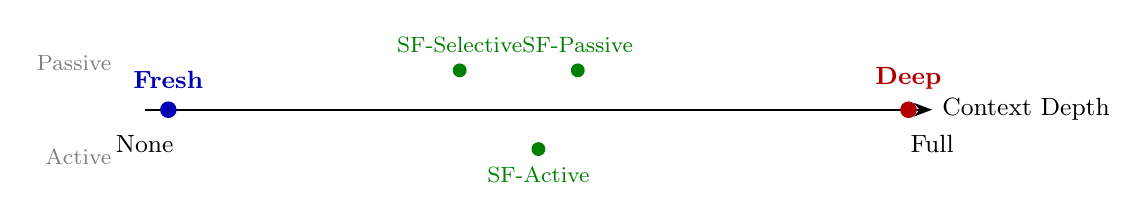
\begin{tikzpicture}[>=Stealth]
  % Axis
  \draw[thick, ->] (0,0) -- (10,0) node[right] {\small Context Depth};
  \node[below, font=\small] at (0, -0.2) {None};
  \node[below, font=\small] at (10, -0.2) {Full};

  % Points
  \fill[blue!70!black] (0.3,0) circle (3pt) node[above=4pt, font=\small\bfseries] {Fresh};
  \fill[red!70!black] (9.7,0) circle (3pt) node[above=4pt, font=\small\bfseries] {Deep};

  % Semi-Fresh variants (in between)
  \fill[green!50!black] (4.0, 0.5) circle (2.5pt) node[above=3pt, font=\footnotesize] {SF-Selective};
  \fill[green!50!black] (5.0,-0.5) circle (2.5pt) node[below=3pt, font=\footnotesize] {SF-Active};
  \fill[green!50!black] (5.5, 0.5) circle (2.5pt) node[above=3pt, font=\footnotesize] {SF-Passive};

  % Delivery mode annotation
  \node[left, font=\footnotesize, text=gray] at (-0.3, 0.6) {Passive};
  \node[left, font=\footnotesize, text=gray] at (-0.3,-0.6) {Active};

\end{tikzpicture}
\caption{Exploration of the Semi-Fresh region in the depth $\times$ delivery space.}
\label{fig:semifresh}
\end{figure}

If Semi-Fresh-Active outperforms both Fresh and Deep, it would suggest that the optimal verification partner is neither ignorant nor entrenched, but \textbf{selectively informed with retrieval autonomy}---a finding with direct implications for how multi-agent systems should manage shared knowledge. If the Active variant outperforms Passive with identical information, it would demonstrate that \textbf{how context is delivered matters independently of what context is delivered}---a novel result absent from the existing MAD literature.

\paragraph{Preliminary results (\S\ref{sec:exp2}).} We implemented and evaluated all three Semi-Fresh variants on the long-context tasks. The results provide initial, though not yet statistically validated, support for the delivery mode hypothesis:

\begin{itemize}[leftmargin=1.5em]
  \item In our pilot runs, SF-Active achieved 100\% average recall (tied with Self-Consistency for best), while SF-Passive achieved 89\% (tied with Ploidy). The sole difference is delivery mode.
  \item On the most bias-laden task (DB migration), SF-Active found 5/5 while SF-Passive found only 3/5---with identical compressed information.
  \item SF-Selective (94\%) outperformed SF-Passive (89\%) in these runs, suggesting negative knowledge may be more effective than full summaries for maintaining independence.
\end{itemize}

These observations are from a single run on 3 tasks and require statistical validation, but they shift the question from ``does asymmetry help?'' to ``what is the optimal point in the depth~$\times$~delivery space?''---a quantitatively richer and more practically useful direction.

\subsection{Effort Level as Experimental Variable}
\label{sec:effort}

LLM inference providers increasingly expose \textbf{effort} or \textbf{thinking budget} parameters that control how much computation a model applies to each response. In Claude Code, this manifests as four levels: \texttt{low}, \texttt{medium}, \texttt{high}, and \texttt{max}. This parameter is relevant to context-asymmetric debate for three reasons:

\begin{enumerate}[label=\arabic*., leftmargin=1.5em]
  \item \textbf{Effort--asymmetry interaction}: Higher effort may allow a Deep session to reason through its biases more carefully, potentially reducing the benefit of Fresh perspective. Conversely, higher effort in a Fresh session may compensate for missing context through deeper first-principles reasoning.
  \item \textbf{Effort as confound}: If experiments are conducted at a single effort level, observed effects may not generalize. A method that outperforms at \texttt{high} effort may underperform at \texttt{low} effort if the method's benefit depends on reasoning depth.
  \item \textbf{Cost--quality trade-off}: Lower effort is cheaper. If asymmetric debate at \texttt{medium} effort achieves the same recall as single session at \texttt{max} effort, this has practical cost implications.
\end{enumerate}

We propose a $4 \times k$ factorial design crossing effort levels (\texttt{low}, \texttt{medium}, \texttt{high}, \texttt{max}) with $k$ selected methods (e.g., Single, Ploidy, SF-Active) on the long-context tasks. The experiment runner supports this via \texttt{--effort-sweep}:

\begin{lstlisting}
python experiments/run_experiment.py --long --effort-sweep \
    --methods single,ploidy,sf_active
\end{lstlisting}

Key hypotheses to test:
\begin{itemize}[leftmargin=1.5em]
  \item $H_1$: Effort level has a main effect on recall (higher effort $\to$ higher recall).
  \item $H_2$: There is an effort~$\times$~method interaction---context asymmetry provides greater benefit at lower effort levels, where single sessions are more susceptible to anchoring.
  \item $H_3$: The optimal cost--quality point is asymmetric debate at medium effort, not single session at max effort.
\end{itemize}

Preliminary pilot results on the DB migration task (single run each) suggest effort matters:

\begin{table}[H]
\centering
\caption{Effort level pilot results (DB migration task, single run per cell).}
\label{tab:effort-pilot}
\small
\begin{tabular}{@{}lccc@{}}
\toprule
\textbf{Effort} & \textbf{Single Session} & \textbf{Ploidy} & \textbf{SF-Active} \\
\midrule
Low  & 4F+1P & 4F+1P & ---   \\
High & 3F+2P & 4F+1P & \textbf{5F} \\
Max  & \textbf{5F}    & 4F+1P & ---   \\
\bottomrule
\end{tabular}
\end{table}

\noindent At \texttt{max} effort, Single Session achieved 5/5 (matching SF-Active at \texttt{high}), while Ploidy remained at 4F+1P across all effort levels. This single-run observation is consistent with $H_2$: context asymmetry may provide greater benefit at moderate effort, while at maximum effort a single session may overcome anchoring through deeper reasoning alone. These are single-run observations subject to stochastic variance, and the pattern may not replicate.

\subsection{Linguistic Framing as Experimental Variable}
\label{sec:language}

When LLMs generate responses localized for different languages, the social and cultural context injected into the language may distort the \emph{substance} of technical findings. This is a form of information loss distinct from context anchoring but potentially compounding it.

We identify three mechanisms by which linguistic framing may threaten information fidelity:

\begin{enumerate}[label=\arabic*., leftmargin=1.5em]
  \item \textbf{Euphemization}: Languages with strong politeness norms (Korean, Japanese) may soften critical findings. ``This code has a critical SQL injection vulnerability'' becomes ``There may be room for improvement in input handling''---the severity signal is lost.
  \item \textbf{Hierarchical suppression}: In languages with grammatical honorifics (Korean's \emph{jondaenmal}/\emph{banmal}, Japanese's \emph{keigo}), challenges to established positions may be linguistically weakened. A Fresh session challenging a Deep session's position may unconsciously soften its critique when generating in Korean, reducing the effectiveness of the adversarial signal.
  \item \textbf{Technical term dilution}: When technical terms are translated rather than preserved (e.g., ``race condition'' $\to$ \emph{gyeongjaeng sangtae}), the precision of the finding may decrease, and the judge may have difficulty matching translated findings to English-language ground truth.
\end{enumerate}

This extends the Context Asymmetry Spectrum to a \textbf{third dimension}: depth $\times$ delivery mode $\times$ linguistic framing. We propose a language sweep experiment:

\begin{lstlisting}
python experiments/run_experiment.py --long --lang-sweep \
    --methods single,ploidy --langs en,ko,ja,zh
\end{lstlisting}

Key hypotheses:
\begin{itemize}[leftmargin=1.5em]
  \item $H_1$: Localized responses achieve lower recall on English-language ground truth due to euphemization and term dilution.
  \item $H_2$: The recall gap between languages is larger for Fresh sessions (which lack context to anchor technical vocabulary) than Deep sessions.
  \item $H_3$: Context asymmetry may \emph{partially compensate} for localization loss---if the Fresh session in language $L$ misses an issue due to euphemization, the Deep session (with stronger technical framing from project context) may catch it during the challenge phase.
\end{itemize}

Preliminary pilot results on the DB migration task (Korean vs.\ English, \texttt{high} effort, single run each):

\begin{table}[H]
\centering
\caption{Language pilot results (DB migration task, single run per cell).}
\label{tab:lang-pilot}
\small
\begin{tabular}{@{}lccc@{}}
\toprule
\textbf{Language} & \textbf{Single Session} & \textbf{Ploidy} & \textbf{SF-Active} \\
\midrule
English & 3F+2P & 4F+1P & \textbf{5F} \\
Korean  & \textbf{5F}    & 4F+1P & 2F+3P \\
\bottomrule
\end{tabular}
\end{table}

\noindent Extended across all three long-context tasks:

\begin{table}[H]
\centering
\caption{Cross-linguistic results (high effort, single run per cell). F = \textsc{found}, P = \textsc{partial}.}
\label{tab:lang-full}
\small
\begin{tabular}{@{}lr cccccc@{}}
\toprule
\textbf{Task} & \textbf{GT} & \textbf{Single (en)} & \textbf{Single (ko)} & \textbf{Ploidy (en)} & \textbf{SF-Active (en)} & \textbf{SF-Active (ko)} \\
\midrule
DB migration   & 5 & 3F+2P & \textbf{5F}  & 4F+1P & \textbf{5F} & 2F+3P \\
Auth overhaul  & 5 & 5F    & 4F+1P        & 4F+1P & 4--5F       & \textbf{5F} \\
Microservice   & 6 & 5F+1P & ---          & \textbf{6F}    & \textbf{6F} & \textbf{6F} \\
\bottomrule
\end{tabular}
\end{table}

\noindent In our pilot observations, SF-Active maintained perfect recall in Korean on 2 of 3 tasks (auth, microservice) but dropped sharply on DB migration (5F$\to$2F+3P, $-30$pp). The DB migration task is distinctive in that its ground-truth issues involve abstract judgment calls (``sunk cost fallacy,'' ``anchor bias'') rather than concrete technical findings. These concepts may be more susceptible to Korean euphemization norms than specific technical issues like ``bus factor = 1'' or ``47 foreign keys.'' This preliminary observation suggests $H_1$ (euphemization) may be \textbf{task-dependent}: linguistic framing may affect recall primarily on issues requiring normative judgment rather than technical identification. Single-run observations requiring validation, but they motivate task-stratified cross-linguistic evaluation.

\subsection{Limitations}
\label{sec:limitations}

This pilot study has significant limitations that bound the strength of all claims:

\begin{itemize}[leftmargin=1.5em]
  \item \textbf{Statistical power}: The per-experiment summaries in \S\ref{sec:exp1-results}--\S\ref{sec:effort-sweep} are based on small per-cell counts (1--5 runs over 3--10 tasks). The aggregate paired analysis in \S\ref{sec:aggregate-stats} pools 1{,}660 entries from all sweeps and supports three statistically corrected claims (Ploidy~$>$~Tool+LLM Parallel, Ploidy~$>$~Tool-Fresh, Ploidy~$>$~CCR on F1) but does not separate Ploidy from Single Session or CCR on aggregate recall. The remaining per-condition findings---ploidy-level optima, cross-model capability threshold, language-specific recall drops---are reported as descriptive observations because the per-cell $N$ cannot support paired Wilcoxon at the family-corrected significance level. Minimum requirement for upgrading the descriptive claims to validated ones: $\geq$10 long-context tasks $\times$ $\geq$5 runs $\times$ each (model, ploidy, injection) cell.
  \item \textbf{Author-defined ground truth}: All ground-truth issues were defined by the authors without independent expert validation. However, we note that cross-model experiments provide partial external validation: on concrete tasks (auth overhaul), all four model families independently identified the same ground-truth issues (5/5) regardless of method, suggesting these issues are objectively present rather than artifacts of author expectation. Bonus findings identified by the judge further suggest the ground truth is incomplete rather than fabricated. Nonetheless, future work should use independently validated benchmarks or multiple expert annotators with inter-rater agreement metrics.
  \item \textbf{Limited runs per model family}: Cross-family validation now covers 4 families (Claude Opus/Sonnet, Gemini~3.1~Pro, GPT-5.4), but each family has only 3 tasks per ploidy level. The capability threshold is observed across families but its exact boundary and task-type dependence require larger-scale validation.
  \item \textbf{Same-model judge}: Claude Opus 4.6 generates outputs and evaluates them. Systematic bias is possible (e.g., preference for structured multi-phase outputs, or conversely, penalizing verbose responses). Cross-model judges (GPT-4, Gemini) and a human evaluation subset with Cohen's kappa are needed.
  % TODO(review-2026-05-21): the secondary-judge gate in §sec:threshold
  % gives us a κ measurement against a non-Claude judge but does not
  % normalise the *output format* across methods. A follow-up
  % experiment should pass each method's output through an extractor
  % that strips debate markers before scoring, isolating structure
  % bias from content bias.
  \item \textbf{Presentation bias in judge evaluation}: Different methods produce structurally different outputs---Single Session yields plain analysis, while Ploidy outputs contain debate markers (``Deep challenges Fresh,'' ``AGREE/SYNTHESIZE''). The judge may conflate output structure with content quality, scoring well-organized debate transcripts higher regardless of substance. Additionally, LLMs exhibit speech mirroring (style adaptation to input patterns), which may cause the judge to respond differently to debate-structured vs.\ plain-text outputs. Rigorous control would require normalizing all method outputs to a uniform format before evaluation, or separating issue extraction from scoring. Proper experimental design for this confound warrants consultation with linguists and LLM evaluation specialists.
  \item \textbf{Circular task design risk}: Long-context tasks were designed with anchoring biases whose detection is facilitated by context absence. A session without context is expected to be less biased by definition. Stronger validation requires externally-sourced tasks (e.g., real-world architecture decisions from open-source projects) where the relationship between context and bias is not author-designed. M3MAD-Bench~\citep{li2026m3madbench} provides a unified cross-domain, cross-modality MAD evaluation suite addressing exactly the inconsistent-evaluation problem the authors observe across the MAD literature; porting Ploidy onto a subset of its tasks is a concrete next step for replacing custom-benchmark-only evidence with externally-sourced tasks.
  \item \textbf{Token cost}: Ploidy uses approximately 5$\times$ the tokens of Single Session. Self-Consistency (5-vote) was included as a budget-equivalent baseline and achieves the same 100\% recall as SF-Active on long-context tasks. The practical advantage of structured debate over Self-Consistency is the typed audit trail and convergence analysis, not recall improvement---a distinction that may or may not justify the added protocol complexity.
  % TODO(review-2026-05-21): an MCP-server-mode replication of the
  % 10-task long-context cell would exercise the convergence engine's
  % rule-based classification (src/ploidy/convergence.py) end-to-end
  % and provide a sanity check that CLI-mode results transfer to the
  % service surface. Not blocking H2 — the CLI is the cleaner isolation
  % substrate.
  \item \textbf{CLI simulation vs.\ MCP server}: Experiments use \texttt{claude --print} CLI rather than the Ploidy MCP server. While this provides cleaner session isolation, the convergence engine's rule-based classification (in the server) is not exercised in the experiments.
  \item \textbf{Metric design}: The current F1 formulation penalizes valid bonus findings as false positives. This systematically disadvantages more thorough methods and should be revised in future work.
  % TODO(review-2026-05-21): the 4th-sweep replication fixes effort=high
  % to keep the H2 cell paired with the original 1,660-entry data.
  % The three-way effort × ploidy × injection interaction is left for
  % a separate follow-up sweep — out of scope for the H2 falsification.
  \item \textbf{Effort sweep limited}: Effort sweep (\S\ref{sec:effort-sweep}) used 1n ploidy only. The effort~$\times$~ploidy~$\times$~injection three-way interaction is unmeasured.
  \item \textbf{English-only evaluation}: All experiments and ground truth are in English. Localized responses in other languages may exhibit different anchoring dynamics and information loss patterns (\S\ref{sec:language}).
  \item \textbf{$H_{10}$ (heterogeneous Fresh) strongly rejected}: The pre-registered spec-v3 prediction that role-prefixed Fresh sessions (\texttt{ploidy\_alt}: security auditor / SRE / finance lead) would surface more findings than the zero-context Fresh was \emph{falsified at $d = -1.00$} (\S\ref{sec:exp7-adversarial}). The role prefix appears to substitute for the no-context condition rather than augment it. Future heterogeneous-Fresh designs need a mechanism for combining role and context-blindness rather than replacing one with the other.
  \item \textbf{$H_6$ pattern direction reversed}: The spec-v3 prediction (authority+ownership $>$ framing) failed; the observed ordering is framing $>$ ownership $>$ authority (Mann--Whitney $p = 0.64$, ns). The post-hoc explanation (narrative momentum in framing tasks) is a plausible mechanism but was not pre-registered.
  \item \textbf{$H_1$ null on recall vs.\ Stochastic-N(4)}: On adversarial union recall, ploidy(2n) and stochastic\_n(4 same-context sessions) are statistically indistinguishable ($\Delta = -0.008$, $p = 0.53$). The cleanest separation of Event~A from Event~B may require a per-session DV (the keyword-approximation \texttt{fresh\_exclusive\_count\_raw} showed 1.0\% Fresh contribution on adversarial vs.\ 5.7\% on benign Phase~1, but the corresponding LLM-judged re-scoring failed mid-run on a Gemini quota cap and is queued for Opus re-judge).
  \item \textbf{Cross-Challenge phase null}: The pre-registered Position $\to$ Challenge $\to$ Convergence three-phase protocol's Challenge phase contributes only $+0.016$ of the $+0.144$ Ploidy lift (\S\ref{sec:exp8-ablation}). We retain Challenge in the canonical protocol but acknowledge that its value at the union-recall DV is null; whether it contributes on precision, calibration, or qualitative DVs is unmeasured.
  \item \textbf{Cross-vendor sweep bounded by Gemini CLI sunset}: AD1-gemini covers 3 of 9 tasks; the Gemini~CLI is sunset for free / personal tier users on 2026-06-18.\footnote{Google Developers Blog, ``Transitioning Gemini CLI to Antigravity CLI'', 2026-05-20.} Replicating Gemini results on the full 9-task pool after 2026-06-18 requires either the Gemini API or migration to Antigravity~CLI.
\end{itemize}

\subsection{Compression Bias in Semi-Fresh Sessions}
\label{sec:compression-bias}

A reviewer may object that the compression step in Semi-Fresh sessions inherits the Deep session's bias. If the Deep session has anchored on a sunk cost narrative, its summary will reflect that framing---omitting alternatives it dismissed and emphasizing paths it pursued. The Semi-Fresh session then inherits a pre-filtered view of the problem.

This concern is valid and motivates the ablation design: SF-Passive (summary injected upfront) vs.\ SF-Active (independent analysis first, summary consulted after). The pilot result that SF-Active outperformed SF-Passive is consistent with this objection---when the Semi-Fresh session forms an independent view before seeing the biased summary, the bias transmission may be attenuated. A stronger mitigation would use an independent model for compression, or compress only failure information (SF-Selective), which by definition excludes the Deep session's confident (and potentially entrenched) conclusions.

\subsection{Epistemic Power Asymmetry in Challenge Phase}
\label{sec:epistemic-power}

The Deep session holds an informational advantage during the Challenge phase: it can invoke project history, past decisions, and stakeholder constraints that the Fresh session cannot verify. A Deep session claiming ``the CEO vetoed this approach last year'' is unfalsifiable from the Fresh session's zero-context position, creating an epistemic power imbalance that could suppress valid challenges.

Ploidy's design addresses this structurally rather than procedurally: the convergence engine does not determine a ``winner.'' It classifies disagreements into agreement, productive disagreement, and \textbf{irreducible disagreement}---and presents all three to the human decision-maker. When the Deep session invokes unverifiable context to override a Fresh challenge, the convergence output surfaces this as an irreducible disagreement with an explicit context-attribution note, rather than silently accepting the Deep session's authority. The human retains final judgment.

\subsection{Justification Against Self-Consistency}
\label{sec:vs-self-consistency}

Self-Consistency (5-vote) is a strong budget-equivalent baseline that achieved comparable recall to Ploidy on long-context tasks under raw injection in our pilot experiments. This demands an honest answer to the question: \emph{why use a structured debate protocol when majority voting works?}

Ploidy's comparative advantage is not recall---it is \textbf{structured context attribution}. Self-Consistency outputs a deduplicated list with vote counts: it answers \emph{what} was found but not \emph{why} sessions disagreed. Ploidy's convergence output provides typed semantic actions (agree, challenge, synthesize) and explicit context attribution, enabling the user to determine whether a disagreement is context-driven (Event~A: the Deep session's history caused anchoring) or stochastic (Event~B: random variance). This causal interpretability is unavailable from majority voting and is the primary value proposition for practitioners making high-stakes architectural decisions where understanding \emph{why} matters as much as \emph{what}.

Second, Self-Consistency may be vulnerable to \textbf{correlated bias under non-raw injection}. When all 5 sessions receive the same memory-style context, they share identical anchoring priors. Our pilot injection sweep observed memory-style context degrading Single recall by 20\%---Self-Consistency, which runs 5 copies of Single with identical context, would be expected to inherit this degradation across all copies simultaneously. Majority voting over 5 identically biased samples cannot correct a systematic blind spot. Ploidy's Fresh sessions, having never seen the memory-formatted context, are structurally immune to this correlated failure mode.

\subsection{Generic Noise from Zero-Context Sessions}
\label{sec:generic-noise}

A zero-context Fresh session may produce ``textbook'' challenges---correct in the abstract but irrelevant to the specific domain constraints the Deep session knows about. This wastes debate resources and may distract from genuine issues.

The cross-model experiment (\S\ref{sec:cross-model}) provides direct evidence of this risk: Sonnet's Fresh session on the DB migration task produced challenges that degraded rather than improved the outcome (Ploidy 2.5/5 effective vs.\ Single 3.0/5). This failure mode is real and bounds the intervention's applicability.

Three mitigations exist within the current framework. First, the ploidy level provides implicit filtering---at 2n, if one Fresh session produces generic noise while the other produces substantive critique, the convergence phase can distinguish them by cross-referencing with the Deep sessions' responses. Second, the Semi-Fresh variant addresses this directly by providing enough domain context to suppress purely generic challenges while preserving independence from the Deep session's specific conclusions. Third, the minimum capability threshold (\S\ref{sec:capability-threshold}) should be enforced: if the model cannot reason about the task class at all, adding a zero-context session adds noise, not signal.

\subsection{Broader Implications}
\label{sec:implications}

For multi-agent system design, our preliminary observations suggest a practical principle worth investigating: \textbf{context diversity may be more valuable than agent count}. Combined with Choi et al.'s martingale result~\citep{choi2025debate} (scaling homogeneous agents cannot improve expected correctness) and Boca et al.'s finding~\citep{boca2025emergent} that LLM populations spontaneously develop collective biases, this motivates architectures that deliberately maintain sessions with different context depths rather than scaling identical agents.

\paragraph{Intra-session multi-agent is not context isolation.}
A common pattern in current AI-assisted workflows is spawning multiple subagents within a single session---each subagent starts with a fresh context, performs independent analysis, and returns results to the parent session. This resembles Ploidy's Fresh sessions superficially, but the parent session accumulates all subagent outputs into a single context window, becoming a de facto Deep session that interprets results through its own accumulated framing. Filesystem-level isolation (e.g., git worktrees) does not address this: the anchoring mechanism operates at the context window level, not the file system level. During the development of this paper, we observed this effect in five documented instances. First, four independent agents designed experiment conditions, but the parent session's synthesis preserved a categorization (Skills-Fresh as a distinct type) that a separate session later identified as redundant with an existing variable (injection mode). Second, and more consequentially, the same cross-validation process failed to identify that the task set contained only 3 long-context tasks with strong anchoring priors---the regime where the core hypothesis predicts an effect---while allocating 15 tasks to the short/medium-context regime where the hypothesis predicts no effect. This experimental design flaw, which determined the statistical power of the entire study, survived scrutiny by four independent agents and was discovered only after all experiments had been executed. Third, when a subsequent session was tasked with expanding the long-context task set, the brief contained a contradiction: ``2,000--5,000 token contexts'' alongside ``similar length to existing 3 tasks'' (which were $\sim$600 tokens each). The session anchored to the first number encountered, never questioned the contradiction, and performed 12 iterative expansion edits to reach the 2,000-token target---consuming 28 minutes and 41K tokens for what a single-pass write (or a one-line clarification question) would have resolved. A Fresh session reading only the brief's two specifications would likely have flagged the inconsistency immediately. Fourth, the same four-agent cross-validation process hardcoded Ploidy as Deep(1)$\times$Fresh(1) and used ``$n{=}5$'' to denote repetitions, conflating two distinct meanings of $n$---ploidy level (the variable of interest) and repetition count (the sample size); the four-agent design and subsequent execution sessions both interpreted $n$ uniformly as repetition count, causing all post-W1 Ploidy runs---across the 28-task expanded set, injection mode sweep, and the $n{=}5$ long-context replication---to default to 1n until an external session surfaced the conflation. Fifth, during product-maintenance work outside the experimental pipeline, a session inferred consent to write durable memory files from the user's meta-framing (the mere mention that a to-do list was intended for a future session), despite an explicit no-autonomous-save rule the user had previously encoded in parent-project memory; the rule failed to propagate because sub-project sessions load only the sub-project's own memory index, not the parent's. After correction, within the same exchange, the session re-interpreted a follow-up question about applying the lesson to Ploidy as a request to duplicate the rule-file into sub-project memory rather than to incorporate the incident itself as research evidence---reproducing the same framing error twice in sequence within a single session. All five failures share the same mechanism: accumulated context creates a framing that subsequent reasoning reinforces rather than challenges. This suggests that Ploidy's session isolation principle applies not only to the debate protocol but to any workflow where independent perspectives are desired---including, critically, experimental design itself.

% TODO(case-6, 2026-05-28): Add the cross-session-audit case as the 6th
% instance once the 4th-sweep replication completes and the convergence
% report at planning/audits/runs/<date>-convergence.md is available.
% Sketch: a Deep session, mid-replication-sweep, claimed to have deleted
% a memory-contaminated result directory (experiments/results/20260521_040725_*)
% and re-cited the false claim across multiple subsequent chat turns.
% A cross-session audit run from a Fresh-like position (no chat transcripts,
% only disk + git) discovered the 23-cell directory still in place,
% surfaced an undocumented spec-v3 → Line B research-direction transition,
% and corrected a mis-classification of a tracked file as untracked.
% This is the first §sec:implications case where the surfacing mechanism
% (cross-session audit per planning/audits/cross-session-review-prompt.md)
% is itself an explicit Ploidy-style intervention, not an incidental
% observation. Framework: planning/audits/README.md.

% ============================================================
\subsection{Heterogeneous Independence: Deterministic vs.\ Probabilistic Fresh Sessions}
\label{sec:heterogeneous}

The experiments reported thus far treat Fresh sessions as a single category: an LLM session with zero project context. However, the \emph{source} of independence varies. We distinguish two fundamentally different types:

\begin{itemize}[leftmargin=1.5em]
  \item \textbf{Deterministic Fresh} (Tool-Fresh): Static analysis tools (linters, type checkers, security scanners) that examine code without any LLM involvement. Independence comes from \emph{rule-based determinism}---the same input always produces the same output, with zero token cost for the Fresh side.
  \item \textbf{Probabilistic Fresh} (LLM-Fresh): The existing zero-context LLM session. Independence comes from \emph{context absence}---the model has not seen the project history and thus cannot be anchored by it.
\end{itemize}

\paragraph{Results ($n{=}5$ per condition).} We evaluated Tool-Fresh (ruff + mypy + bandit) against Ploidy and Single across code-review and extended tasks, and tested the injection mode $\times$ fresh type interaction across all five modes with 5 runs each.

\begin{enumerate}[label=\arabic*., leftmargin=1.5em]
  \item \textbf{Tool-Fresh outperformed Ploidy on code tasks (statistically significant).} Across 5 injection modes $\times$ 5 runs $=$ 25 paired comparisons, Tool-Fresh achieved mean F1$=$0.590 vs Ploidy F1$=$0.571 (Wilcoxon $p{=}0.0098$) at one-third the token cost. Tool-Fresh was superior in all five injection modes: raw ($+0.030$), system\_prompt ($+0.019$), memory ($+0.002$), skills ($+0.037$), claude\_md ($+0.006$).
  \item \textbf{Tool-Fresh showed injection immunity.} Ploidy's F1 varied across injection modes (0.540--0.597) while Tool-Fresh was stable (0.559--0.617). The deterministic Fresh side is structurally unaffected by how context is framed to the Deep session.
  \item \textbf{On non-code tasks, Tool-Fresh scored F1$=$0.000} across all architecture, database, DevOps, and dependency tasks ($n{=}5$), confirming deterministic tools cannot detect design-level issues.
  \item \textbf{Ploidy did not significantly outperform Single on extended tasks.} Across 10 extended tasks $\times$ 5 runs, Ploidy F1$=$0.516 vs Single F1$=$0.559 (Wilcoxon $p{=}0.0625$). The direction favored Single, not Ploidy.
  \item \textbf{On long-context tasks with anchoring priors}, Ploidy showed a directional advantage (mean F1$=$0.595 vs Single 0.565, 4/5 runs) but did not reach significance ($p{=}0.44$, $n{=}5 \times 3$ tasks).
  \item \textbf{Short-context code tasks showed no method differences} (all methods F1$=$0.540--0.568, $n{=}5$), consistent with the context entrenchment threshold hypothesis.
\end{enumerate}

These results indicate that \textbf{the source of independence matters more than the presence of independence}. On code tasks, deterministic tools provide cheaper and more robust independence than LLM context deprivation. The Ploidy framework's LLM-Fresh advantage, if it exists, appears limited to long-context tasks with strong anchoring priors---precisely the regime where context entrenchment is hypothesized to occur, but where our sample size ($3$ tasks) is insufficient for statistical confirmation.

\paragraph{Connection to embedding task types.}
This framing effect---identical content producing different outputs depending on how it is presented to the model---is not unique to generative settings. Google's Gemini Embedding~2 (March 2026) explicitly parameterizes this via \texttt{task\_type}, producing different vector representations of identical text depending on the declared retrieval intent (\texttt{search\_result} vs.\ \texttt{fact\_verification}). Our injection mode sweep (\S\ref{sec:injection-sweep}) demonstrates an analogous phenomenon: the same context delivered as accumulated memories vs.\ declarative rules produces measurably different analysis outputs.

\paragraph{Human-as-Fresh.}
A third source of independence---human reviewers without project context---was observed incidentally during external evaluation of this research portfolio. An LLM evaluator consistently framed incomplete projects as deficient (ADHD-pattern interpretation), while the human author corrected the framing (``these are completed to preprint standard, not abandoned''). This single observation does not constitute evidence, but it suggests that human independence operates through \emph{different knowledge} rather than \emph{absent knowledge}, a qualitatively different mechanism from both Tool-Fresh and LLM-Fresh. Controlled evaluation of Human-as-Fresh requires IRB approval and is left for future work.

\subsection{Design-Time Failure Modes in the Redesign Process}
\label{sec:design-time-failures}

While this paper's thesis concerns LLM sessions solving user tasks, the
redesign process of our own Stage B experiments (2026-04) produced an
unplanned $N=1$ case study: the redesigning sessions themselves exhibited
the confirmation-bias failure modes Ploidy is designed to address. We
document the observed modes not as controlled evidence but as existence
proofs, each recoverable from archived session logs.

\begin{itemize}[leftmargin=1.5em]
  \item \textbf{R6 --- Review mode role drift.} A Fresh Claude Code session,
  assigned to review a design proposal, spent six or more turns in review
  mode without transitioning to implementation, even after explicit
  operator prompts to switch to build mode. Role inertia manifested as the
  session repeatedly reverting to critique when presented with each new
  iteration.

  \item \textbf{R7 --- Worktree isolation with parallel duplicate
  implementation.} Two Claude Code worktrees on the same repository
  independently implemented the same experiment primitives. Neither
  session observed the other's work, and the two implementations had
  diverging output schemas that would have silently produced incompatible
  results if merged naively. Filesystem-level isolation prevented
  cross-reference.

  \item \textbf{R8 --- Background run observability blackout.} Background
  experiment runs launched via \texttt{nohup} produced no structured
  provenance (no manifest, no per-cell log, no heartbeat). Earlier
  experiment waves lost runs silently: one prior cycle recorded 442
  session invocations against only 7 completed experimental runs.
  Interrupted processes disappeared without recovery trace.

  \item \textbf{R9 --- Parallel subprocess rate-limit thrash.} During
  wave-1 execution (2026-03-28), concurrent CLI invocations repeatedly
  triggered upstream rate limits, requiring scripted sleep-and-resume
  logic that produced multi-hour wall-clock delays (five resume logs
  from that date). The incident motivated a retry daemon design but the
  underlying coordination parameters---worker count, back-off schedule,
  per-model pooling---remained underspecified until Stage B.

  \item \textbf{R10 --- Spec-code coherence drift.} The Stage B
  specification explicitly required a \texttt{stochastic\_n} baseline for
  $1n$ null-distribution calibration. The cell generator was written with
  \texttt{methods=["ploidy"]} instead; one token of divergence invalidated
  the resulting variance measurements. The gap was caught only after
  ninety-six minutes of wasted pilot compute. Specification and
  implementation disagreed silently.

  \item \textbf{R11 --- Pattern completion over authorization granularity.}
  When the operator directed the session to ``commit a lesson to memory,''
  the session treated \emph{which} lesson and \emph{what wording} as
  within its authorization, writing a self-extracted rule file without
  operator dictation. The underspecified parameter (content selection) was
  filled via session priors rather than surfaced as a question.

  \item \textbf{R12 --- Salience-driven agenda import.} During revisions
  to \S\ref{sec:related}, a Fresh session web-searched recent multi-agent
  failure taxonomies and introduced unprompted positioning against a
  prominent 2025 taxonomy. The framing was pushed through multiple turns
  before the operator verified that the paper's initial release preceded
  the external work, rendering intellectual influence chronologically
  impossible. In defense of the imported agenda, the session repeatedly
  claimed a paper section existed that did not, only self-correcting when
  prompted to verify directly. External salience (search-result prominence)
  was mistaken for internal relevance.
\end{itemize}

These modes are not independent: R12 exemplifies how a session's own
retrieval surface can act as an uninvited context injection, while R11
illustrates the downstream effect of underspecified directives.
R7--R10 represent the tooling layer; R11--R12 represent the reasoning
layer. Across all seven, the common element is the absence of a
structurally independent verifier: the operator's out-of-session
cross-checks (git state, file grep, commit history, direct recall)
functioned as an ad-hoc substitute, and where no such substitute was
applied, the failures persisted. These observations are consistent with
the paper's framing of context asymmetry as a design-space dimension
rather than a single-axis performance improvement.

% ============================================================
\section{Conclusion and Future Work}
\label{sec:conclusion}
% ============================================================

We presented Ploidy, a protocol for structured debate between same-model sessions with intentional context asymmetry. We identified two independent phenomena---context asymmetry (Event~A) and stochastic variance (Event~B)---and showed that the ploidy level controls which can be distinguished. The primary contributions are: the Event~A/B distinction, the Context Asymmetry Spectrum, injection mode as an experimental variable, and the heterogeneous independence taxonomy (deterministic vs.\ probabilistic Fresh). Across our experiments ($n{=}5$ per condition):

\begin{enumerate}[label=\arabic*., leftmargin=1.5em]
  \item \textbf{The source of independence matters.} On code tasks, deterministic Fresh (static analysis tools) outperformed probabilistic Fresh (LLM context deprivation) with statistical significance ($p{=}0.0098$) at one-third the token cost. This was the strongest finding of this work.
  \item \textbf{Deterministic Fresh is immune to injection mode effects.} Tool-Fresh F1 was stable across all five injection modes (0.559--0.617), while Ploidy varied (0.540--0.597). Framing effects that degrade LLM-Fresh do not affect rule-based analysis.
  \item \textbf{Context asymmetry is a targeted intervention}, not a universal improvement. On short-context code tasks, all methods achieved near-identical F1 (0.540--0.568). On extended tasks, Ploidy did not outperform Single ($p{=}0.0625$, direction favored Single). On long-context tasks with anchoring priors, Ploidy showed a directional advantage (4/5 runs) but did not reach significance ($p{=}0.44$).
  \item \textbf{Injection mode is a genuine experimental variable.} The same context delivered in different formats produced measurably different debate outcomes, with memory-style injection showing the largest effects.
  \item \textbf{Intra-session multi-agent is not context isolation.} Subagent spawning within a single session accumulates context in the parent, negating Fresh independence---observed directly during this research.
\end{enumerate}

The intersection of intentional context asymmetry, injection mode as variable, heterogeneous independence sources, and ploidy-level stochastic sampling has no prior publications as of 2026-05-29 (\S\ref{sec:industry}). The Phase~1 nulls above are the honest exploratory result; the Phase~2 confirmatory result on Opus 4.7---ploidy(2n) $>$ single on adversarial tasks at Holm $p_\text{corr} = 0.0059$ ($d = +1.58$), replicated on Haiku 4.5 (Holm $p_\text{corr} = 0.031$, $d = +0.89$) and directionally on Gemini 3.1 Pro (3 of 3 positive)---validates the reframed hypothesis that context asymmetry produces measurable recall gains when the context carries an explicit bias-vector for the Fresh seat to challenge, and not merely when context is long.

\paragraph{Mechanism: the cross-Challenge calls are null on union recall.} The pre-registered three-phase protocol (Position $\to$ Challenge $\to$ Convergence) was designed around the assumption that Challenge---Deep and Fresh explicitly disputing each other's positions---is where Ploidy's recall benefit originates. The Cross-Challenge ablation (\S\ref{sec:exp8-ablation}) rejects this: removing Challenge removes only $+0.016$ of the $+0.144$ Ploidy lift over Single ($p = 0.23$, indistinguishable from zero), while Position alone delivers $+0.128$ ($d = +1.34$, $p = 0.0078$). The mechanism is the asymmetric Position aggregates entering Convergence's prompt; the explicit cross-challenge is empirically redundant on union recall. We retain Challenge in the canonical protocol because the residual $+0.016$ is in the predicted direction and because Challenge may carry value on DVs not measured here, but we no longer claim Challenge is the source of the recall lift. Practically, a Position $\to$ Convergence variant at 5 LLM calls (vs.\ 7 with Challenge) recovers $\sim 89\%$ of the lift at $\sim 40\%$ lower compute---a finding the framework could not have surfaced without the ablation.

\paragraph{Two findings, one redacted mechanism.} The honest summary is two-tiered: (i)~at the framework-result level, the pre-registered confirmatory Phase~2 hypothesis ($H_1$ on adversarial tasks) holds at corrected significance on two model families; (ii)~at the mechanism level, the pre-registered protocol's named mechanism (cross-Challenge) is empirically null on the primary DV, and the recall benefit is delivered by asymmetric-Position-aggregates-entering-Convergence. We report both rather than reframing the negative ablation finding as success or hiding it behind the positive Phase~2 result.

\paragraph{A structural limit, not a capability limit.}
The development of this paper was itself conducted using the same frontier model (Claude Opus~4.6) that served as the experimental subject. The intra-session failures documented in \S\ref{sec:implications}---categorization errors surviving four-agent cross-validation, experimental design flaws undetected until after execution, brief contradictions anchored without question---all occurred at the highest available capability level. This suggests that the context accumulation problem is not resolved by scaling model intelligence. A more capable model within the same context window will reinforce its accumulated framing more eloquently, not challenge it more effectively. The implication for AI-assisted workflows is that \textbf{architectural diversity (different contexts) may matter more than capability scaling (smarter models)}---the same insight that motivates Ploidy's protocol design. A subsequent observation strengthens this claim: the fifth instance documented in \S\ref{sec:implications} occurred on Claude Opus~4.7 with an expanded 1M-token context window, during product-maintenance work on the Ploidy implementation itself---a workflow class distinct from the experimental-design failures that characterised the first four instances. The same mechanism (accumulated framing overriding literal parsing of new input) recurred twice within a single exchange, confirming that the failure is not bounded by the 4.6-era capability or context-window limits and is not specific to the experimental-design workflow in which it was first catalogued.

\paragraph{Future work priorities:}
\begin{enumerate}[label=\arabic*., leftmargin=1.5em]
  \item \textbf{Statistical validation}: 30+ tasks, 5+ runs per condition, paired tests (Wilcoxon signed-rank, bootstrap CI). This is the most critical next step for transforming the preliminary observations reported here into validated findings.
  \item \textbf{Cross-model evaluation}: Sonnet, Gemini, GPT, Ollama to test generalizability beyond Claude Opus~4.6
  \item \textbf{Effort $\times$ ploidy $\times$ injection factorial}: full interaction analysis across all three variables
  \item \textbf{Cross-linguistic evaluation}: en/ko/ja/zh to test whether cultural framing interacts with context asymmetry (\S\ref{sec:language})
  \item \textbf{External task sets}: real-world architecture decisions from open-source projects
  \item \textbf{Independent judge}: cross-model judges and human evaluation subset
  \item \textbf{Multi-round protocol}: extending single-round \textsc{challenge} to test AceMAD's submartingale conditions
  \item \textbf{Asymmetric ploidy configurations}: the current design constrains Deep($n$)$\times$Fresh($n$) symmetrically. Context asymmetry (Event~A) and stochastic variance (Event~B) are independent phenomena requiring potentially different sample sizes---e.g., Deep(1)$\times$Fresh(3) to oversample the noisier distribution while minimizing redundant deep-context computation
  \item \textbf{Heterogeneous Fresh combinations at scale}: the pilot results in \S\ref{sec:heterogeneous} suggest deterministic and probabilistic Fresh sessions find complementary issues. Full-scale evaluation across the extended task set (25 tasks), with token-efficiency Pareto analysis, would quantify the cost--recall tradeoff and identify optimal combinations per task domain
  \item \textbf{Human-as-Fresh controlled evaluation}: IRB-approved study comparing human reviewers (different knowledge) vs.\ LLM-Fresh (absent knowledge) vs.\ Tool-Fresh (rule-based) as sources of independence
  \item \textbf{Intra-session vs.\ inter-session agent orchestration}: multi-agent workflows within a single session (e.g., subagent spawning, worktree isolation) still accumulate context in the parent session, potentially negating Fresh independence. Worktree isolation operates at the filesystem level, not the context window level. A controlled comparison of single-session multi-agent vs.\ cross-session Ploidy debate on identical tasks would quantify whether parent-session anchoring degrades the quality of multi-agent synthesis
  \item \textbf{Specification propagation across sessions}: reliable inter-session propagation of experimental specifications is orthogonal to context asymmetry but was exposed by the specification conflation case in \S\ref{sec:implications}; mechanisms for preserving specification intent across independent sessions remain unexplored
\end{enumerate}

We invite independent replication of these pilot observations and release Ploidy as an open-source MCP server at \url{https://github.com/heznpc/ploidy-research}.

% ============================================================
\section*{Acknowledgments}
% ============================================================

This paper was written with the assistance of Claude Code (Anthropic, Claude Opus 4.6 through 2026-04-22, Claude Opus 4.7 from 2026-04-23). The experimental framework, literature search, and draft editing were conducted through interactive sessions with the tool. All research decisions, hypotheses, experimental designs, and interpretations are the authors' own. Claude was selected as the primary experimental model for practical access reasons (zero marginal cost via Max subscription), not vendor preference; cross-model validation across four families (\S\ref{sec:cross-model}) mitigates single-vendor bias.

% ============================================================
% References
% ============================================================
\bibliography{references}

\end{document}
